\section{Technical Lemmas}
\label{apx:results}
\begin{lemma}[\cite{levy2024online}]
\label{lem:good_event}
Let $\delta \in (0,1)$. Let $t_{i,n} \in [T]$ be the time at which packet type $i\in [K]$ is selected for the $n$-th time. Let $\mathcal{E}(\delta)$ be the \textit{good event} under which:
\begin{itemize}
    \item $0 < LCB_{i,t_{i,1}} < \ldots < LCB_{i,t_{i,n}} \le \mu_i$ for every $i \in [K]$ and $n \in [T]$.
    \item $\mu_i \le UCB_{i,t_{i,n}} < \ldots < UCB_{i,t_{i,1}} = 1$ for every $i \in [K]$ and $n \in [T]$.
    \item $UCB_{i,t_{i,n}}-LCB_{i,t_{i,n}}\le 2\beta_{i, t_{i,n}}$ for every $i \in [K]$ and $n \in [T]$.
\end{itemize}
Then, we have $\mathbb{P}(\mathcal{E}(\delta))\ge 1- \delta$.
\end{lemma}

\begin{lemma}
\label{lem:bound_comparison}
Let $i,j\in[K]$ be packet types with means $\mu_i>\mu_j$ and gap $\Delta_{i,j}:=\mu_i-\mu_j>0$. Then, on the event $\mathcal{E}\!\left(\frac{1}{T}\right)$, the event
\[
\Bigl\{\mathrm{UCB}_{j,t}>\mathrm{UCB}_{i,t}\Bigr\}\;\cap\;\Bigl\{i,j\in\mathcal{B}_t\Bigr\}\;\cap\;\Bigl\{j\text{ is scheduled at time }t\Bigr\}
\]
can occur at most
\[
Q_{i,j}\;=\;\frac{8\,\ln T}{\Delta_{i,j}^2}
\]
times.
\end{lemma}

\begin{proof}
We work under the event $\mathcal{E}\!\left(\frac{1}{T}\right)$. 
Fix any round $t$ for which $i,j\in\mathcal{B}_t$ and arm $j$ is scheduled. Consider $\mathrm{UCB}_{j,t}\;>\;\mathrm{UCB}_{i,t}$.
Unfolding the indices and adding and subtracting the true means,
\begin{align*}
\widehat\mu_{j,t}+\sqrt{\frac{2\ln T}{N_{j,t}}}
\;>\;
\widehat\mu_{i,t}+\sqrt{\frac{2\ln T}{N_{i,t}}}
&\;\;\Longrightarrow\;\;
\bigl(\mu_j-(\mu_j-\widehat\mu_{j,t})\bigr)+\sqrt{\frac{2\ln T}{N_{j,t}}}\\
&\hspace{3.3cm}>\;
\bigl(\mu_i-(\mu_i-\widehat\mu_{i,t})\bigr)+\sqrt{\frac{2\ln T}{N_{i,t}}}.
\end{align*}
Hence $(\mu_j-\widehat\mu_{j,t})\le \sqrt{2\ln T/N_{j,t}}$ and $(\mu_i-\widehat\mu_{i,t})\ge -\sqrt{2\ln T/N_{i,t}}$, so the previous display yields
\[
\mu_j- \sqrt{\frac{2\ln T}{N_{j,t}}}+\sqrt{\frac{2\ln T}{N_{j,t}}}
\;>\;
\mu_i- \sqrt{\frac{2\ln T}{N_{i,t}}}+\sqrt{\frac{2\ln T}{N_{i,t}}},
\]
that is,
\[
\mu_i-\mu_j
\;\le\; 2\,\sqrt{\frac{2\ln T}{N_{j,t}}}.
\]
Equivalently,
\begin{equation}\label{eq:key}
N_{j,t}\;\le\;\frac{8\,\ln T}{\Delta_{i,j}^2}.
\end{equation}

Now observe that each time the event
\[
\Bigl\{\mathrm{UCB}_{j,t}>\mathrm{UCB}_{i,t}\Bigr\}\cap\Bigl\{i,j\in\mathcal{B}_t\Bigr\}\cap\Bigl\{j\text{ is scheduled}\Bigr\}
\]
occurs, the counter $N_{j,t}$ increases by one. Thus, if this event were to occur more than $m$ times, then there would exist a round $t$ with $N_{j,t}>m$ at which it still occurs. Choosing any $m\ge \dfrac{8\,\ln T}{\Delta_{i,j}^2}$ contradicts \eqref{eq:key}. In particular, taking 
\[
m\;=\;\frac{8\,\ln T}{\Delta_{i,j}^2}
\]
is valid (it is a looser threshold), and therefore the event in the statement can occur at most $Q_{i,j}=8\,\ln T/\Delta_{i,j}^2$ times.
\end{proof}
The following lemma includes some properties of $\widehat{p}_{ab,t}$, which are crucial for the analysis of \algrtwo. Let $\mathcal{E}(\delta)$ be the \textit{good event} under which all confidence intervals hold simultaneously for every type $i \in [K]$ and round $t \in [T]$.
\begin{restatable}[Properties of $\phat$]{lemma}{phatprop}
    Let $a_t^* \in \argmax_{a \in V_t^*} w_a$ and $b_t^* \in \argmax_{b \in B_t^*} w_b$, where $V_t^*$ is the set of pending packets with deadline $t$ for \opt at time $t$, and $B_t^*$ is the set of the ones having deadline greater than $t$. 
    %Consider Equation \eqref{eq:p_hat} and the decision rule of \algrtwo. 
    Then, under the good event $\mathcal{E}_T(\delta)$, the followings hold for every $t \in [T]$:
    \begin{subequations} \label{eq:phat_props}
    \begin{align}
        5\phat a_t &\ge 4 a_t^* - b_t^* - 10\beta_{a_t, t}  \label{eq:phat_1}\\[3pt]
        5(\phat a_t + \qhat b_t) &\ge 4b_t^* - 10 \beta_{a_t,t} -8\beta_{b_t, t}\label{eq:phat_2}\\[3pt]
        5\phat a_t + 2\qhat b_t &\ge 4a_t^*- 10 \beta_{a_t,t} \label{eq:phat_3} \\[3pt]
        5\phat a_t + 2\qhat b_t &\ge b_t^* - 10 \beta_{a_t,t}-2\beta_{b_t, t} \label{eq:phat_4}
    \end{align}
\end{subequations}
\end{restatable}
\begin{proof}
    Under the \textit{good event}, all confidence intervals contain the true mean. Thus $LCB_{i,t} \le \mu_i \le UCB_{i,t}$ and $LCB_{i,t}+2\beta_{i,t} \ge \mu_i \ge UCB_{i,t}-2\beta_{i,t}$ for every $i \in [K]$ and $t \in [T]$.
    \begin{enumerate}[align=left]
    \item [Proof of Equation \eqref{eq:phat_1}]
    \begin{align*}
        5\phat a_t &\ge 5\phat \ucba - 10 \phat \beta_{a_t,t} \\
        &\ge 4\ucba-\lcbb-10\betaa \\
        &\ge 4\ucbaopt - \lcbbopt -10\betaa \\
        &\ge 4 a_t^* - b_t^* -10 \betaa.
    \end{align*}
    \item [Proof of Equation \eqref{eq:phat_2}] 
    \begin{align*}
        5(\phat a_t + \qhat b_t) &\ge 5(\phat \ucba + \qhat \lcbb)- 10\phat \betaa \\
        &\ge 5(\phat \ucba + \qhat \lcbb)- 10\phat \betaa  \\
        &\ge 4\lcbb -10\betaa \\
        &\ge 4\ucbb -10\betaa - 8\betab \\
        &\ge 4 b_t^* -10\betaa - 8\betab.
    \end{align*}
    \item [Proof of Equation \eqref{eq:phat_3}] 
    \begin{align*}
        5\phat a_t + 2\qhat b_t &\ge 5\phat \ucba + 2\qhat \lcbb - 10\phat \betaa \\
        &\ge 4\ucba - 10\phat \betaa  \\
        &\ge 4a_t^* -10\betaa.
    \end{align*}
    \item [Proof of Equation \eqref{eq:phat_4}] 
    \begin{align*}
        5\phat a_t + 2\qhat b_t &\ge 5\phat \ucba + 2\qhat \lcbb - 10\phat \betaa \\
        &\ge \lcbb - 10\phat \betaa  \\
        &\ge \ucbb - 10\betaa - 2\betab \\ 
        &\ge b_t^* - 10\betaa - 2\betab.
    \end{align*}
\end{enumerate}
\end{proof}
\section{Omitted Proofs}
\label{apx:proofs}
\reductionMABS*
\begin{proof}
    By the definition of $K$-armed sleeping bandits of \cite{kleinberg2010regret}, there exist $K$ types of actions and at every round $t \in [T]$ an adversary selects a subset $\mathcal{A}_t \subseteq [K]$ to propose to the learner. Actions selected in time $t$ are only available in that round, and unless the adversary selects them again, are not available anymore after $t$, since at most one action can be played per round. In $1$-bounded $K$-OPSD, we can just ignore packets with the same type except for one: the packets with the same type are indistinguishable and only one of them can eventually be played. For every action $a \in \mathcal{A}_t$, we create a buffer $\mathcal{B}_t$ s.t. there exists at least one packet $p_a$ of type $a \in \mathcal{B}_t$. Then, no matter how many copies of $p_a$ there are in the buffer, the decision space is always the same and is equivalent to the size of the minimal buffer, which is actually $\mathcal{A}_t$.
\end{proof}
\subsection{Deterministic Algorithms}
%%%%%%%%%%%%%%%%%%%%%%%%%%%%%%%%%%%%%%%%%%%%%%%%%%%%%%%
\begingroup
  \setcounter{lemma}{0}
  \renewcommand\thelemma{3.\arabic{lemma}}
\begin{lemma}[Sleeping Bandits are a special case of $K$-OPSD]
Every $1$-bounded instance of the $K$-OPSD problem can be reduced to a $K$-armed Sleeping Bandit problem, and viceversa.
\end{lemma}
\endgroup
\begin{proof}
    By the definition of $K$-armed sleeping bandits of \cite{kleinberg2010regret}, there exist $K$ types of actions and at every round $t \in [T]$ an adversary selects a subset $\mathcal{A}_t \subseteq [K]$ to propose to the learner. Actions selected in time $t$ are only available in that round, and unless the adversary selects them again, are not available anymore after $t$, since at most one action can be played per round. In $1$-bounded $K$-OPSD, we can just ignore packets with the same type except for one: the packets with the same type are indistinguishable and only one of them can eventually be played. For every action $a \in \mathcal{A}_t$, we create a buffer $\mathcal{B}_t$ s.t. there exists at least one packet $p_a$ of type $a \in \mathcal{B}_t$. Then, no matter how many copies of $p_a$ there are in the buffer, the decision space is always the same and is equivalent to the size of the minimal buffer, which is actually $\mathcal{A}_t$.
\end{proof}
%%%%%%%%%%%%%%%%%%%%%%%%%%%%%%%%%%%%%%%%%%%%%%%%%%%%%%%
\algedflearnBound*
\begin{proof}
    We call $f_t$ the packet sent by \alg in $t$, and $j_t$ the packet sent by \opt in $t$. We also call $h_t$ the packet in the buffer of ALG at time $t$ such that $h_t \in \argmax_{h\in \mathcal{B}_t} UCB_{h,t}$. To lighten the notation, we let the name of the packet coincide with its type. 

    We consider the \textit{charging scheme} in which $j_t$ is charged to its copy in the \alg schedule up to $t$ if it exists, otherwise it is charged to $f_t$. 

    For $\delta \in (0,1)$, define the uniform ``good'' event
    \[
    \mathcal{E}\!\left(\delta\right)
    \;:=\;\bigcap_{k=1}^K\;\bigcap_{n=1}^{T}
    \left\{\left|\widehat{\mu}_{k,n}-\mu_k\right|\le \sqrt{\frac{2\ln \delta^{-1}}{n}}\right\},
    \]
    where $\widehat{\mu}_{k,n}$ denotes the empirical mean of arm $k$ after $n$ samples. Lemma \ref{lem:good_event} states that the good event holds with probability at least $1-\delta$. Let $\delta = \frac{1}{T}$. Since
    \begin{align*}
        \mathbb{E}[R_{\Phi,T}^{\text{\algedflearn}}] &= \mathbb{E}\left[R_{\Phi,T}^{\text{\algedflearn}}|\mathcal{E}(\delta)\right]\mathbb{P}\left(\mathcal{E}(\delta)\right) + \mathbb{E}\left[R_{\Phi,T}^{\text{\algedflearn}}|\mathcal{E}(\delta)^C\right]\mathbb{P}\left(\mathcal{E}(\delta)^C\right) \\
        &\le \mathbb{E}\left[R_{\Phi,T}^{\text{\algedflearn}}|\mathcal{E}(\delta)\right]\mathbb{P}\left(\mathcal{E}(\delta)\right) + \mathcal{O}(1),
    \end{align*}
    we focus on bounding the first addendum under the good event.
    
    We proceed by cases.

    \paragraph{Case $1$: $f_t$ only receives one charge}Ideally, we want to show that $f_t$ receives a charge that is at most $\Phi f_t$.
    \paragraph{Case $1a$: $f_t$ receives a charge from $f_t$} Then the total charge is obviously $f_t$. No $\Phi$-regret is accrued in this case.
    \paragraph{Case $1b$: $f_t$ receives a charge from $j_t$} Then, \alg hasn't send $j_t$ before $f_t$. This implies that $j_t \in \mathcal{B}_t$ and that $\Phi UCB_{j_t,t} < UCB_{h_t,t} \le \Phi UCB_{f_t,t}$, and $UCB_{j_t,t} < UCB_{f_t,t}$. If $j_t \le f_t$, then the total charge is trivially bounded by $f_t$. If $j_t > f_t$, the instantaneous $\Phi$-regret can be bounded as
    $$
    j_t - \Phi f_t < UCB_{j_t,t} - \Phi f_t< \Phi UCB_{f_t,t} - \Phi f_t\le \Phi \beta_{f_t,t}.
    $$
    Since $UCB_{j_t,t} < UCB_{f_t,t}$ can occur at most $Q_{j_t,f_t}= \frac{8\ln T}{\Delta_{j_t,f_t}^2}$ times (Lemma \ref{lem:bound_comparison}), the total $\Phi$-regret accrued in this case is bounded as
    $$
    \Phi \sum_{t=1}^{Q_{j_t,f_t}} \beta_{f_t,t} \le \frac{8\Phi \ln T}{\Delta_{j_t,f_t}}.
    $$
    \paragraph{Case $2$: $f_t$ receives a charge from $j_t$ and a charge from $f_t$} In this case, $j_t \in \mathcal{B}_t$ and \opt has scheduled $f_t$ after time $t$. Also, $\Phi UCB_{j_t,t} < UCB_{h_t,t} \le \Phi UCB_{f_t,t}$. We have to distinguish two cases.
    \paragraph{Case $2a$: $d_{f_t}=t+2$} In this case, we have $UCB_{f_t,t}=UCB_{h_t,t}$. If $\Phi j_t \leq f_t$, we have $j_t+f_t \le \left(1+\Phi^{-1}\right)f_t = \Phi f_t$, and no $\Phi$-regret is accrued. If $\Phi j_t > f_t$, we have that $\Phi UCB_{j_t,t} \le UCB_{f_t,t}$ can occur at most $Q_{j_t,t}^\Phi = \frac{8\ln T}{\left(\Delta_{f_t,j_t}^\Phi\right)^2}$ times (Lemma \ref{lem:bound_comparison}), where $\Delta_{f_t,j_t}^\Phi > 0$. The instantaneous $\Phi$-regret can be bounded as
    $$
    (j_t + f_t) - \Phi f_t< UCB_{j_t,t} - \Phi^{-1} f_t < \Phi^{-1}UCB_{f_t,t} - \Phi^{-1} f_t \le \Phi^{-1} \beta_{f_t,t}.
    $$
    The total $\Phi$-regret accrued in this case is bounded as
    $$
    \Phi^{-1} \sum_{t=1}^{Q_{j_t,f_t}^{\Phi}} \beta_{f_t,t} \le \frac{8\ln T}{\Delta_{f_t,j_t}^\Phi},
    $$
    with $\Delta_{f_t,j_t}^\Phi > 0$.
    \paragraph{Case $2b$: $d_{f_t}<t+2$} In this case, we have $d_{h_t}=t+2$ and $d_{j_t}\le d_{f_t}$, since the schedule of \opt is ordered with ascending deadlines. Since $f_t$ is played by \opt after $t$, and of course before $t+2$, it must be that $d_{f_t}=t+1$. So we consider the couple of packets scheduled by \alg in $t$ and $t+1$, a bound the $\Phi$-regret accrued in these two rounds jointly. Note that $f_{t+1}$ can receive a charge only from its copy, since \opt plays $f_t$ in $t+1$ and is charged to $f_t$ itself. Moreover, $\Phi UCB_{f_t,t} \ge UCB_{h_t,t}$. If $\Phi j_t < f_t$, we have $(j_t+f_t+f_{t+1})-\Phi (f_t + f_{t+1}) < (\Phi^{-1}f_t+f_t+f_{t+1})-\Phi(f_t+t_{t+1}) < 0$, and there is no $\Phi$-regret.
    If $\Phi j_t \ge f_t$, the instantaneous $\Phi$-regret can be bounded as 
    \begin{align*}
        (j_t+f_t+f_{t+1})-\Phi (f_t + f_{t+1}) &< UCB_{j_t,t} - \Phi^{-1}(f_t+f_{t+1}) \\
        & \le \Phi^{-1} \frac{1}{2} 2UCB_{h_t,t} - \Phi^{-1}(f_t+f_{t+1}) \\
        & \le \frac{1}{2\Phi} \Phi(UCB_{f_t,t} + UCB_{f_{t+1},t}) - \Phi^{-1}(f_t+f_{t+1}) \\
        & \le \frac{3}{2}(\beta_{f_t,t}+\beta_{f_{t+1},t}).
    \end{align*}
    Since $j_t \in \mathcal{B_t}$, this situation can occur until $UCB_{j_t,t} < UCB_{f_t,t}$, thus at most $Q_{j_t,f_t}$ times (Lemma \ref{lem:bound_comparison}). The total $\Phi$-regret accrued in this case is bounded as
    $$
    \frac{3}{2}\sum_{t=1}^{Q_{j_t,f_t}} \beta_{f_t,t} \le \frac{8\Phi\ln T}{\Delta_{j_t,f_t}}.
    $$
    Summing up all the possible regrets sources for every round, and recombining by packet type, yields the first result:
    \begin{align*}
        R_{\Phi,T}^{\text{\algedflearn}} \le \mathcal{O} \left(\sum_{t=1}^T \left(\frac{1}{\Delta_{j_t,f_t}} + \frac{1}{\Delta_{f_t,j_t}^\Phi} \right) \ln T\right) \\
        \le \mathcal{O}\left(K\sum_{i =1}^{K - 1} \frac{\ln T}{\Delta_{i, i+1}} + \sum_{\substack{i,j \in [K]\\ \Delta_{i,j}^\Phi > 0}} \frac{\ln T}{\Delta_{i,j}^\Phi}\right).
    \end{align*}
    The second bound can be obtained by noting that, every time a packet $f_t$ is played, the instantaneous $\Phi$-regret at round $t$ can be bounded by $\beta_{f_t,t}$. Summing up for every packet type $i\in [K]$, and for the number of times a packet of type $i$ has been scheduled, we get
    $$
    \sum_{i \in [K]} \sum_{n=1}^{N_{i,T}} \beta_{i,t_{i,n}} \le \widetilde{\mathcal{O}}\left( \sum_{i \in [K]}\sqrt{N_{i,T}} \right) \le \widetilde{\mathcal{O}}\left(\sqrt{KT}\right),
    $$ 
    where $t_{i,n}$ is the round in which a packet of type $i$ has been scheduled for the $n$-th time.
\end{proof}
\upperboundtheta*
\begin{proof}
    We analyze separately the two types of possible epochs, \emph{i.e.} the ones ending with $b_{t+\ell}$ (\textit{first type}) and the ones ending with $v_{t+\ell}$ (\textit{second type}), where $\ell$ will be used to indicate the length of an epoch. Note that, by construction, any epoch can be at most $K$ rounds long, \emph{i.e.} $\ell \le K$. We have to show two things: (1) every epoch starts with the buffer of \opt being entirely contained in the buffer of \algtheta, thus \opt has no advantage gained from previous epochs; (2) $\Gopt^E \le \theta_K \Galgtheta^E$ for every epoch $E$, where $\Gopt^E$ indicates the gain of \opt inside epoch $E$, and $\Galgtheta^E$ indicates the gain of \algtheta inside epoch $E$. These two facts combined yield a global competitive ratio of $\theta_K$.
    \paragraph{(1) \algtheta starts every epoch with a larger or equal buffer to \opt.} We prove this fact by allowing for a \textit{stronger} \opt. In particular, at the end of every epoch, we allow \opt to send additional packets until its buffer is entirely contained in the buffer of \algtheta. 
    \paragraph{(1a) $\{v_t, \ldots, b_{t+\ell}\}$-type epochs.} Consider an epoch $E$ starting in $t$ and ending in $t+\ell$ of the first type, then we have:
    \begin{align*}
        \Galgtheta^E = \sum_{j=0}^{\ell-1} v_{t+j} + b_{t+\ell}.
    \end{align*}
    Assuming that \opt starts with a buffer that is smaller of equal than the one of \algtheta, we upper bound its gain inside epoch $E$ as
    \begin{align}
    \label{eq:gopt_bound_i}
        \Gopt^E \le \sum_{j=0}^{\ell} b_{t+j} + v_{t+\ell},
    \end{align}
    which is the best possible gain inside epoch $E$ since $b_{t+j}>v_{t+j}$ for every $j<\ell$ by construction, $v_{t+\ell}+b_{t+\ell}\ge b_{t+\ell}$. We allowed \opt to schedule an extra packet w.r.t. to \algtheta, which is $v_{t+\ell}$. This way, when epoch $E$ terminates, the following epoch starts with the buffer of \opt contained in the one of \algtheta. 
    \paragraph{(2a) $\{v_t, \ldots, v_{t+\ell}\}$-type epochs} Consider an epoch $E$ starting in $t$ and ending in $t+\ell$ of the second type, then we have:
    \begin{align*}
        \Galgtheta^E = \sum_{j=0}^{\ell} v_{t+j}.
    \end{align*}
    Assuming that \opt starts with a buffer that is smaller of equal than the one of \algtheta, we upper bound its gain inside epoch $E$ as
    \begin{align}
    \label{eq:gopt_bound_ii}
        \Gopt^E \le \sum_{j=0}^{\ell-1} b_{t+j} + v_{t+\ell},
    \end{align}
    which is the best possible gain inside epoch $E$ since $b_{t+j}>v_{t+j}$ for every $j<\ell$ by construction, and $v_{t+\ell}\ge b_{t+\ell}$. When epoch $E$ terminates, the following epoch starts with the buffer of \opt contained in the one of \algtheta. 
    \paragraph{(2) Bounding the competitive ratio of \algtheta in every epoch.} We now prove that, given an epoch $E$ of any type, $\Gopt \le \theta_K\Galgtheta^E$.
    \paragraph{(2a) $\{v_t, \ldots, b_{t+\ell}\}$-type epochs.} Consider an epoch $E$ starting in $t$ and ending in $t+\ell$ of the first type, then we have:
    \begin{align}
    \label{eq:comp_ratio_theta_i}
        \theta_K\Galgtheta^E-\Gopt^E \ge \theta_K\sum_{j=0}^{\ell-1}v_{t+j} + \theta_K b_{t+\ell} - \sum_{j=0}^\ell b_{t+j} - v_{t+\ell},
    \end{align}
    which follows by Equation \eqref{eq:gopt_bound_i}. Our goal is to prove that the RHS of Equation \eqref{eq:comp_ratio_theta_i} is nonnegative for any choice of the sequences $\{v_{t+j}\}_{j=0}^\ell$ and $\{b_{t+j}\}_{j=0}^\ell$. The epoch termination conditions of \algtheta, together with the definitions of $v_{t+j}$ and $b_{t+j}$, impose a set of constraints on these sequences:
    \begin{align}
        v_{t+j}&\ge b_{t+j-1} ,~~ 1 \le j\le K-1, \label{eq:constraints_i}\\
        b_{t+j}&\ge v_{t+j},~~~~ j\ge 0, \label{eq:constraints_ii}\\
        v_{t+j} &\ge \frac{x_j}{x_{j+1}}b_{t+j},~~ 0 \le j \le \ell-1, \label{eq:constraints_iv} \\
        v_{t+\ell} &\le \frac{x_\ell}{x_{\ell+1}}b_{t+\ell}, \label{eq:constraints_v} 
    \end{align}
    where \eqref{eq:constraints_i} follows from the definition of $v_{t+j}$, \eqref{eq:constraints_ii} follows from the epoch termination conditions of \algtheta, and \eqref{eq:constraints_iv} and \eqref{eq:constraints_v} follow from the decision rule of \algtheta (and with the notational convention that $x_0=1$ and $x_K = x_{K-1}$). An important consequence of these conditions is that both $v_{t+j}$ and $b_{t+j}$ are strictly increasing sequences.

    Intuitively, to prove that under these constraints the RHS of Equation \eqref{eq:comp_ratio_theta_i} is nonnegative, we look at it from the perspective of a constrained minimization problem, and show that the feasible minimum set the RHS to $0$. In particular, note that both the objective function \eqref{eq:comp_ratio_theta_i} and the constraints \eqref{eq:constraints_i}-\eqref{eq:constraints_v} are linear in the parameters $v_{t+j}$ and $b_{t+j}$. Thus, the minimum must be in one of the edges of the decision space defined by the constraints. We now define an edge sequence $\widetilde{v}_{t+j}$ and $\widetilde{b}_{t+j}$ where inequalities are tight and the RHS of \eqref{eq:comp_ratio_theta_i} is $0$. Let $s>0$ be any scale parameter (the problem is homogeneous and the sign does not change with rescaling). Then, set
    \begin{align}
        \widetilde{b}_t&=s, \label{eq:edge_i}\\
        \widetilde{v}_t&=s(\theta_K-1), \label{eq:edge_ii}\\
        \widetilde{v}_{t+j}&=\widetilde{b}_{t+j-1},~~~ j\ge 1, \label{eq:edge_iii}\\
        \widetilde{v}_{t+j}&=\frac{x_j}{x_{j+1}}\widetilde{b}_{t+j},~~~ 0\le j\le \ell. \label{eq:edge_iv}
    \end{align}
    A direct implication of \eqref{eq:edge_i}-\eqref{eq:edge_iv} is that 
    \begin{align*}
        \widetilde{v}_{t+j} &= \widetilde{b}_{t+j-1} =\frac{x_{j}}{x_{j-1}}\widetilde{v}_{t+j-1} = \frac{x_j}{x_0} \widetilde{v}_t =s(\theta_K-1) x_j, \\
        \widetilde{b}_{t+j} &=\frac{x_{j+1}}{x_{j}}\widetilde{v}_{t+j} = \frac{x_{j+1}}{x_0} \widetilde{v}_t =s(\theta_K-1) x_{j+1}. \\
    \end{align*}
    We rearrange \eqref{eq:comp_ratio_theta_i}, plug the edge sequence and write
    \begin{align*}
        \theta_K\sum_{j=0}^{\ell-1}\widetilde{v}_{t+j} &+ \theta_K \widetilde{b}_{t+\ell} - \sum_{j=0}^\ell \widetilde{b}_{t+j} - \widetilde{v}_{t+\ell} = \sum_{j=0}^{\ell-1}(\theta_K \widetilde{v}_{t+j}-\widetilde{b}_{t+j})+(\theta_K-1)\widetilde{b}_{t+\ell}-\widetilde{v}_{t+\ell} \\
        &= s(\theta_K-1) \left[\theta_K(1+\ldots+x_{\ell-1}+x_{\ell+1}) - (x_1 + \ldots + 2x_\ell + x_{\ell+1}) \right] = 0,
    \end{align*}
    which is a direct consequence of the definition of $\{x_j\}_{j=0}^{K - 1}$ as a solution to \eqref{eq:system}. We proved that the sequences $\{\widetilde{v}_{t+j}\}_{j=0}^\ell$ and $\{\widetilde{b}_{t+j}\}_{j=0}^\ell$ are feasible and make all the constraints tight. This step of the proof can be concluded by noting that these edge sequences are actually the minimizer of the RHS of \eqref{eq:comp_ratio_theta_i}: the objective is linear with a positive coefficient in $\{v_{t+j}\}_{j=0}^{\ell-1}$ and $b_{t+\ell}$, and we set the minimum possible values for those (all lower bounds became equalities); the objective is linear with a negative coefficient in $\{b_{t+j}\}_{j=0}^{\ell-1}$ and $v_{t+\ell}$, and we set the maximum possible values for those (all upper bounds became equalities). Thus, the term cannot be reduced anymore and it is nonnegative for any feasible sequence of values, and $\Gopt^E\le \theta_K\Galgtheta^E$.
    \paragraph{(2b) $\{v_t, \ldots, v_{t+\ell}\}$-type epochs.} We closely follow the argument developed in the previous step. Consider an epoch $E$ starting in $t$ and ending in $t+\ell$ of the first type, then we have:
    \begin{align}
    \label{eq:comp_ratio_theta_ii}
        \theta_K\Galgtheta^E-\Gopt^E \ge \theta_K\sum_{j=0}^{\ell}v_{t+j} - \sum_{j=0}^{\ell-1} b_{t+j} - v_{t+\ell},
    \end{align}
    which follows by Equation \eqref{eq:gopt_bound_ii}. Our goal is to prove that the RHS of Equation \eqref{eq:comp_ratio_theta_ii} is nonnegative for any choice of the sequences $\{v_{t+j}\}_{j=0}^\ell$ and $\{b_{t+j}\}_{j=0}^\ell$. Constraints \eqref{eq:constraints_i}-\eqref{eq:constraints_iv} still hold, in addition we have
    \begin{align}
        v_{t+\ell} &\ge b_{t+\ell}, \label{eq:constraints_vi},
    \end{align}
    which follows from the epoch termination condition of \algtheta. As before, we need to prove that the RHS of   \eqref{eq:comp_ratio_theta_ii} is nonnegative under any sequence satisfying the constraints.

    We use the same constrained optimization argument as before, and define and edge sequence which makes the constraints tight:
    \begin{align}
        \widetilde{b}_t&=s, \label{eq:edge_i2}\\
        \widetilde{v}_t&=s(\theta_K-1), \label{eq:edge_ii2}\\
        \widetilde{v}_{t+j}&=\widetilde{b}_{t+j-1},~~~ j\ge 1, \label{eq:edge_iii2}\\
        \widetilde{v}_{t+j}&=\frac{x_j}{x_{j+1}}\widetilde{b}_{t+j},~~~ 0\le j\le \ell-1,  \label{eq:edge_iv2} \\
        \widetilde{v}_{t+\ell}&=\widetilde{b}_{t+\ell}, \label{eq:edge_v2}.
    \end{align}
    We now rewrite the RHS of \eqref{eq:comp_ratio_theta_ii} and plug the edge sequences to obtain:
    \begin{align*}
        \theta_K\sum_{j=0}^{\ell}\widetilde{v}_{t+j} &- \sum_{j=0}^{\ell-1} \widetilde{b}_{t+j} - \widetilde{v}_{t+\ell} = \sum_{j=0}^{\ell-1}(\theta_K\widetilde{v}_{t+j}-\widetilde{b}_{t+j})+(\theta_K-1)\widetilde{v}_{t+\ell} \\
        &= s(\theta_K-1)\left[\theta_K(1+\ldots+x_{\ell})-(x_1+\ldots+2x_{\ell})\right] \ge 0,
    \end{align*}
    which is a direct consequence of the definition of $\{x_j\}_{j=0}^{K - 1}$ as a solution to \eqref{eq:system}. We proved that the sequences $\{\widetilde{v}_{t+j}\}_{j=0}^\ell$ and $\{\widetilde{b}_{t+j}\}_{j=0}^\ell$ are feasible and make all the constraints tight. This step of the proof can be concluded by noting that these edge sequences are actually the minimizer of the RHS of \eqref{eq:comp_ratio_theta_ii}: the objective is linear with a positive coefficient in $\{v_{t+j}\}_{j=0}^{\ell}$, and we set the minimum possible values for those (all lower bounds became equalities); the objective is linear with a negative coefficient in $\{b_{t+j}\}_{j=0}^{\ell-1}$, and we set the maximum possible values for those (all upper bounds became equalities). Thus, the term cannot be reduced anymore, and it is nonnegative for any feasible sequence of values, and $\Gopt^E\le \theta_K\Galgtheta^E$.

    Putting all together completes the proof.
\end{proof}
%%%%%%%%%%%%%%%%%%%%%%%%%%%%%%%%%%%%%%%%%%%%%%%%%%%%%%%
\upperboundthetalearn*
\begin{proof}
    The proof follows the argument of the previous one with the addition of optimism. We work under the good event $\mathcal{E}(\delta)$. Due to \algthetalearn epoch termination conditions, all the packets in \opt buffer at the start of an epoch must also be contained in \algthetalearn buffer. We already proved this in the proof of Proposition 4, and the same argument still holds. What we prove now is that the $\theta_K$-regret accrued inside an epoch is bounded by the sum of the widths of the confidence intervals of the packets selected by \algthetalearn.
    \paragraph{(a) $\{v_t, \ldots, b_{t+\ell}\}$-type epochs.} Consider an epoch $E$ starting in $t$ and ending in $t+\ell$ of the first type.  
    Then
    \begin{align*}
        \mathbb{E}[\Gopt^E] \le \sum_{j=0}^{\ell} UCB_{b_{t+j},t} + UCB_{v_{t+\ell},t},
    \end{align*}
    which is an overestimation of the total reward that any algorithm can achieve within the epoch, due to epoch termination conditions of \algthetalearn. Note that under the good event, all confidence intervals contain the true mean, for every packet type and time $t\in [T]$. We want to lower bound the following:
    \begin{align}
        \theta_K\mathbb{E}[\Galgthetalearn^E]&-\mathbb{E}[\Gopt^E] \ge \theta_K\sum_{j=0}^{\ell-1}v_{t+j} + \theta_K b_{t+\ell} - \sum_{j=0}^\ell UCB_{b_{t+j},t} - UCB_{v_{t+\ell},t} \notag \\
        &\ge \theta_K\sum_{j=0}^{\ell-1}UCB_{v_{t+j},t} + \theta_K UCB_{b_{t+\ell},t} - \sum_{j=0}^\ell UCB_{b_{t+j},t} - UCB_{v_{t+\ell},t}+ \label{eq:comp_ratio_thetalearn_i}\\
        &\qquad- 2\theta_K \sum_{j=0}^{\ell-1}\beta_{v_{t+j},t} - 2\theta_K\beta_{b_{t+\ell},t}.\notag
    \end{align}
    We show that \eqref{eq:comp_ratio_thetalearn_i} is lower bounded by $0$. From the \algthetalearn perspective, the UCBs are equivalent to the actual weights. \algthetalearn behaves exactly like \algtheta, and the UCBs satisfy the same constraints. Minimizing \eqref{eq:comp_ratio_thetalearn_i} under the UCB constraints is exactly equivalent to minimize \eqref{eq:comp_ratio_theta_i} under the set of constraints defined in \eqref{eq:constraints_i}-\eqref{eq:constraints_v}. Thus, substituting the UCBs with the actual values and following the same argument of the proof of Proposition 4, step (2a), we get that \eqref{eq:comp_ratio_thetalearn_i} is nonnegative for every sequence of UCBs. 

    Thus, in epoch $E$, we have
    \begin{align}
        \theta_K\mathbb{E}[\Galgthetalearn
        ^E]&-\mathbb{E}[\Gopt^E] \ge - 2\theta_K \sum_{j=0}^{\ell-1}\beta_{v_{t+j},t} - 2\theta_K\beta_{b_{t+\ell},t}.\label{eq:comp_ratio_thetalearn_i_betas}
    \end{align}

    \paragraph{(b) $\{v_t, \ldots, v_{t+\ell}\}$-type epochs.} Consider an epoch $E$ starting in $t$ and ending in $t+\ell$ of the second type. Then
    \begin{align*}
        \mathbb{E}[\Gopt^E] \le \sum_{j=0}^{\ell-1} UCB_{b_{t+j},t} + UCB_{v_{t+\ell},t},
    \end{align*}
    which is an overestimation of the total reward than any algorithm can achieve inside the epoch, due to epoch termination conditions of \algthetalearn. Note that under the good event all confidence intervals contain the true mean, for every packet type and time $t\in [T]$. We want to lower bound the following:
    \begin{align}
        \theta_K\mathbb{E}[\Galgtheta^E]&-\mathbb{E}[\Gopt^E] \ge \theta_K\sum_{j=0}^{\ell}v_{t+j} - \sum_{j=0}^{\ell-1} UCB_{b_{t+j},t} - UCB_{v_{t+\ell},t} \notag \\
        &\ge \theta_K\sum_{j=0}^{\ell}UCB_{v_{t+j},t} - \sum_{j=0}^{\ell-1} UCB_{b_{t+j},t} - UCB_{v_{t+\ell},t}+ \label{eq:comp_ratio_thetalearn_ii}\\
        &\qquad- 2\theta_K \sum_{j=0}^{\ell}\beta_{v_{t+j},t}.\notag
    \end{align}
    We show that \eqref{eq:comp_ratio_thetalearn_ii} is lower bounded by $0$. From the \algthetalearn perspective, the UCBs are equivalent to the actual weights. \algthetalearn behaves exactly like \algtheta, and the UCBs satisfy the same constraints. Minimizing \eqref{eq:comp_ratio_thetalearn_ii} under the UCB constraints is exactly equivalent to minimize \eqref{eq:comp_ratio_theta_ii} under the set of constraints defined in \eqref{eq:constraints_i}-\eqref{eq:constraints_iv} and \eqref{eq:constraints_vi}. Thus, substituting the UCBs with the actual values and following the same argument of the proof of Proposition 4, step (2b), we get that \eqref{eq:comp_ratio_thetalearn_ii} is nonnegative for every sequence of UCBs. 

    Thus, in epoch $E$, we have
    \begin{align}
        \theta_K\mathbb{E}[\Galgthetalearn^E]&-\mathbb{E}[\Gopt^E] \ge - 2\theta_K \sum_{j=0}^{\ell}\beta_{v_{t+j},t}.\label{eq:comp_ratio_thetalearn_ii_betas}
    \end{align}
    \paragraph{Bounding the Confidence Intervals.} We proved, through \eqref{eq:comp_ratio_thetalearn_i_betas} and \eqref{eq:comp_ratio_thetalearn_ii_betas}, that the per-epoch $\theta_K$-regret is upper bounded by the sum of the widths of the confidence intervals of the packet types selected during that epoch. Let $N_{i,T}$ be the number of times a packet of type $i\in [K]$ has been selected up to time $T$, and $K_E$ be the set of packet types selected during epoch $E$. Also, let $t_E$ the starting time of epoch $E$.
    
    It is important to notice that, due to the constraints enforced on the UCBs of the selected packets, every packet type can only be selected at most once during an epoch. This is a consequence of the fact that the UCBs of the selected packets are strictly increasing during an epoch, and the UCBs are computed at the begin and kept fixed through $E$. 
    
    To complete the proof, we sum over the epochs:
    \begin{align*}
        \mathbb{E}[\Gopt]-\theta_K\mathbb{E}[\Galgthetalearn] &= \sum_{E}\mathbb{E}[\Gopt^E]-\theta_K\mathbb{E}[\Galgthetalearn^E] \\
        &\le 2\theta_K\sum_{E} \sum_{i \in K_E} 
        \beta_{i,t_E} \\
        &\le 2\theta_K \sum_{i \in [K]} \sum_{j=1}^{N_{i,T}}\beta_{i,t_{i,j}} \\
        &\le  2c\theta_K \sum_{i \in [K]} \sum_{j=1}^{N_{i,T}}\sqrt{\frac{\ln \frac{KT}{\delta}}{j}} \le \widetilde{\mathcal{O}}\left(\sqrt{KT}\right),
    \end{align*}
    where the $\widetilde{\mathcal{O}}$ only hides universal constants and logarithmic terms.

    Setting $\delta=\frac{1}{T}$, the good event holds with probability at least $1-\frac{1}{T}$ (Lemma \ref{lem:good_event}):
    \begin{align*}
        \mathbb{E}[R_{\theta_K,T}^{\text{\algthetalearn}}] &= \mathbb{E}[R_{\theta_K,T}^{\text{\algthetalearn}}|\mathcal{E}(\delta)]\mathbb{P}\left(\mathcal{E}(\delta)\right) + \mathbb{E}[R_{\theta_K,T}^{\text{\algthetalearn}}|\mathcal{E}(\delta)^C]\mathbb{P}\left(\mathcal{E}(\delta)^C\right) \\
        &\le \mathbb{E}[R_{\theta_K,T}^{\text{\algthetalearn}}|\mathcal{E}(\delta)] + T\frac{1}{T} \\
        &\le \widetilde{\mathcal{O}}\left(\sqrt{KT}\right).
    \end{align*}
\end{proof}
%%%%%%%%%%%%%%%%%%%%%%%%%%%%%%%%%%%%%%%%%%%%%%%%%%%%%%%
% \begin{remark}[Instance-Dependent Guarantees of \texttt{AUER} and \algthetalearn in $K$-OPSD.]
%     In this work, we only reported worst-case style regret guarantees, with regret upper bounds that only depend on $K$ and $T$. In stochastic bandits literature, however, it is very common to also state \textit{instance-dependent} guarantees, \emph{i.e.}, regret upper bounds that depend on $T$ and the \textit{gaps} between the expected rewards of the actions, like $\Delta_{i,j} \coloneqq  \mu^i-\mu_j$. As it is beyond the scope of this work, we do not state any instance-dependent result, but we remark that those can be conveniently derived for both \texttt{AUER} and \algthetalearn in $K$-OPSD. By adapting the argument of Lemma 9 of \cite{kleinberg2010regret}, it is possible to recover $\alpha$-regret upper bounds that depend on $\Delta_{j,j+1}$, for every $j \in [K]$.
% \end{remark}
%%%%%%%%%%%%%%%%%%%%%%%%%%%%%%%%%%%%%%%%%%%%%%%%%%%%%%%%
\lowerbound*
\begin{proof}
    Through the whole proof, we will refer to $\theta, x_1, \ldots, x_{K - 1}$ as the solution to system \ref{eq:system}. Note that $\theta < \Phi$ for every finite $K$. As the construction is very complex, for the sake of clarity, we start by proving the lower bound on a smaller problem for $\theta_K = \theta_2 = \sqrt{2}$. The full proof (generalized to an arbitrary $K$) can be found in the appendix.
    
    \paragraph{Lower Bound for $\theta_2$-regret.}
    We start by introducing some quantities. Note that $\theta_2 = \sqrt{2}$. Then, let $\delta=\frac{1}{\sqrt{T}}$, $\epsilon = \frac{1}{2\sqrt{T}}$, $\sigma = \frac{4}{\theta_2-1}$, $c = \frac{\theta_2-1}{8}$. Finally, let $X_0 \sim \mathcal{N}(1,\sigma)$ and $X_1 \sim \mathcal{N}(x_1, \sigma)$. Let \alg be an arbitrary, deterministic algorithm.

    \begin{figure}
        \centering
        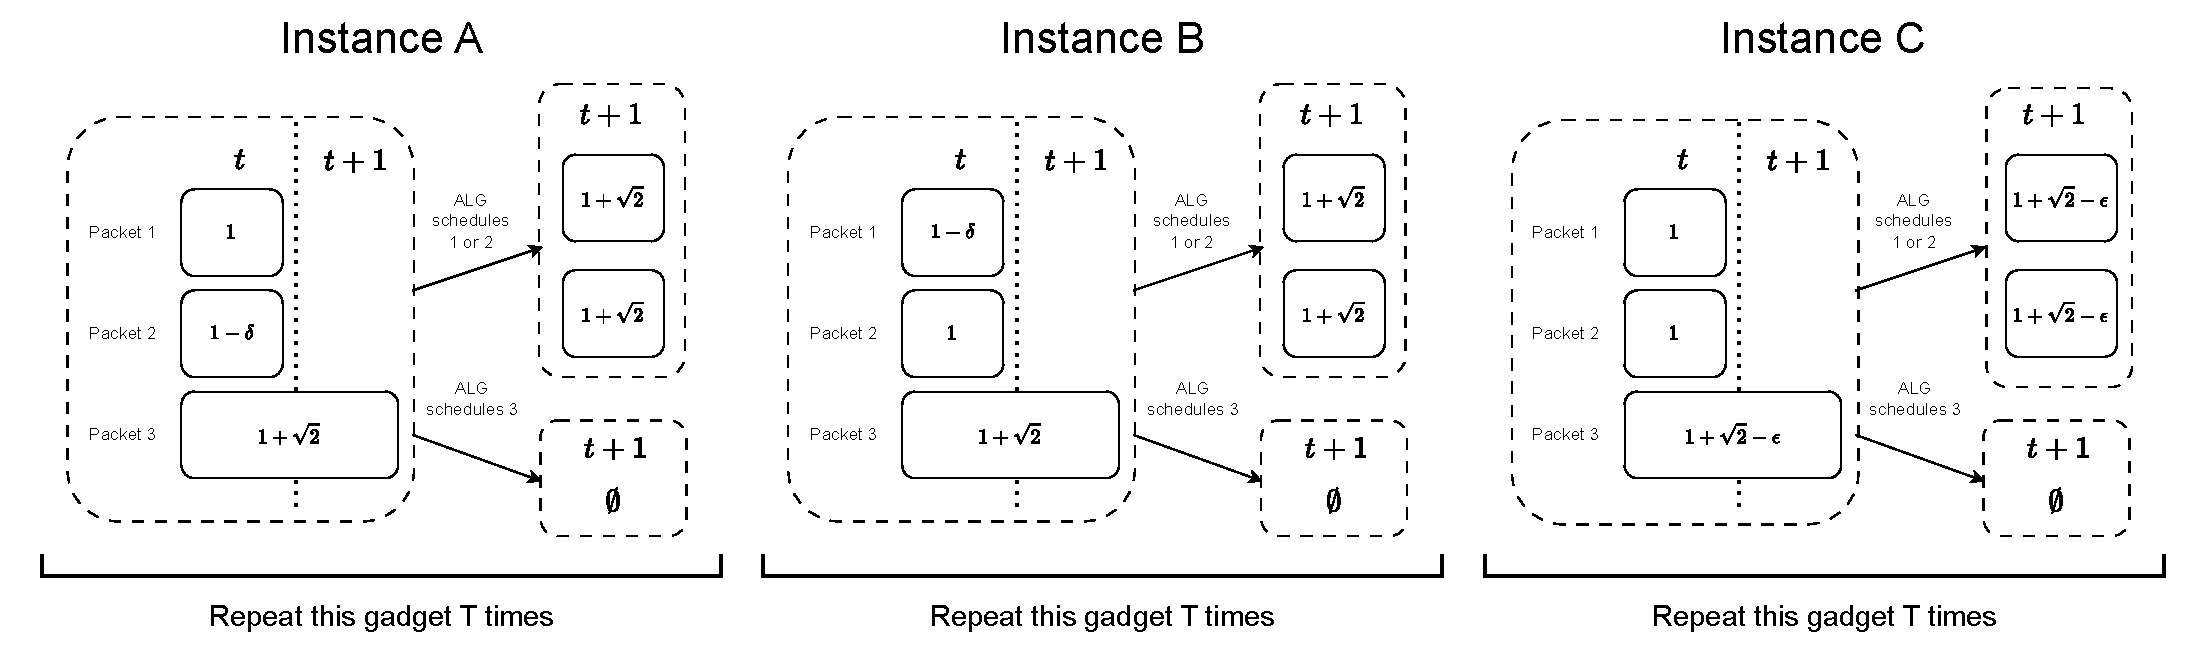
\includegraphics[width=\linewidth]{images/lowerbounds.drawio.pdf}
        \caption{Exemplification of the lower bounds instances. Each gadget (of length two) is repeated $T$ times. What happens in the second round of a gadget depends on the action of \alg in the first.}
        \label{fig:lowerbounds}
    \end{figure}
    
    We consider three instances. Each instance is constructed by repeating a \textit{gadget} for $T$ times. A gadget is a sub-problem that is self-contained; in our case, a gadget is composed of two subsequent rounds, starting from the first. Thus, the total number of rounds will be $2T$. In Figure \ref{fig:lowerbounds}
    
    Instance \texttt{A} is constructed by repeating the following gadget $T$ times: in the first round $t$ of the gadget (\emph{i.e.}, the odd rounds) we have $\mathcal{B}_t = \{(r_1 = t, d_1 = t, X_0, c_1 = 1), (r_2 = t, d_2=t, X_0-\delta, c_2 = 2), (r_3=t, d_3=t+1, X_1, c_3 = 3)\}$; in the second round $t+1$ of the gadget (\emph{i.e.}, the even rounds) we have $\mathcal{B}_{t+1} = \emptyset$ if \alg sent the packet of type $3$ in $t$, and $\mathcal{B}_{t+1} = \{(r_3=t, d_3=t+1, X_1, c_3 = 3), (r_3=t, d_3=t+1, X_1, c_3 = 3)\}$ if \alg sent a packet of type $1$ or $2$ in $t$. Intuitively, \alg is faced with two expiring packets (one having a slightly worse mean reward) and one packet that can also be sent in the following round. If \alg sends the latter, no more packets arrive, and the $\theta_2$-regret w.r.t. to \opt would be $r_2^A = 0$ (by the definition of $\theta_2$ and $x_1$). If \alg acts greedily and sends one of the former, then a copy of the third packet arrives and the expected $\theta_2$-regret w.t. to \opt would be $r_1^A=0$ by scheduling the first and $\widetilde{r}_1^A=\delta\theta_K$ by scheduling the second.

    Instance \texttt{B} is analogous to \texttt{A}, with the difference that we flip type $1$ and type $2$. As a consequence, $r_1^B = \widetilde{r}_1^A$ and $\widetilde{r}_1^B = 0$.

    Instance \texttt{C} is constructed by repeating the following gadget $T$ times: in the first round $t$ of the gadget (\emph{i.e.}, the odd rounds) we have $\mathcal{B}_t = \{(r_1 = t, d_1 = t, X_0, c_1 = 1), (r_2 = t, d_2=t, X_0, c_2 = 2), (r_3=t, d_3=t+1, X_1-\epsilon, c_3 = 3)\}$; in the second round $t+1$ of the gadget (\emph{i.e.}, the even rounds) we have $\mathcal{B}_{t+1} = \emptyset$ if \alg sent the packet of type $3$ in $t$, and $\mathcal{B}_{t+1} = \{(r_3=t, d_3=t+1, X_1-\epsilon, c_3 = 3), (r_3=t, d_3=t+1, X_1-\epsilon, c_3 = 3)\}$ if \alg sent a packet of type $1$ or $2$ in $t$. Intuitively, \alg is faced with two identical expiring packets (even if \alg doesn't know this) and one packet that can also be sent in the following round. If \alg sends the latter, no more packets arrive, and the$\theta_2$-regret w.r.t. to \opt would be $r_2^C = (\theta_2-1)\epsilon$ (by the definitions of $\theta_2$ and $x_1$). If \alg acts greedily and sends one of the former, then a copy of the third packet arrives and the expected $\theta_2$-regret w.r.t. to \opt would be $r_1^C=\widetilde{r}_1^C=(\theta_2-2)\epsilon < 0$.

    Now we show that, no matter what the algorithm does, it is not possible to achieve $\mathcal{O}\left(\sqrt{T}\right)$ $\theta_2$-regret in \texttt{A} and \texttt{C} without achieving $\Omega\left(\sqrt{T}\right)$ $\theta_2$-regret in \texttt{B}. We call $N_{1,T}$, $\widetilde{N}_{1,T}$ and $N_{2,T}$ the number of times \alg selected packet type $1$, $2$, and $3$ in the first step of a gadget, respectively. Let's write the expected regrets for every instance:
    \begin{align*}
        \mathbb{E}_A[R_{\theta_2,T}] &= \theta_2\delta\mathbb{E}_A[\widetilde{N}_{1,T}], \\
        \mathbb{E}_B[R_{\theta_2,T}] &= \theta_2\delta\mathbb{E}_B[{N}_{1,T}], \\
        \mathbb{E}_C[R_{\theta_2,T}] &= (\theta_2-2)\epsilon\mathbb{E}_C[{N}_{1,T}+\widetilde{N}_{1,T}] + (\theta_2-1)\epsilon\mathbb{E}_C[N_{2,T}]. \\
    \end{align*}
    We force both $\mathbb{E}_A[R_{\theta_2,T}]$ and $\mathbb{E}_C[R_{\theta_2,T}]$ to be $\mathcal{O}\left(\sqrt{T}\right)$.
    \begin{align*}
        \mathbb{E}_A[R_{\theta_2,T}] &= \theta_2\delta\mathbb{E}_A[\widetilde{N}_{1,T}] \le c\sqrt{T}, \\
        \mathbb{E}_C[R_{\theta_2,T}] &= (\theta_2-2)\epsilon\mathbb{E}_C[{N}_{1,T}+\widetilde{N}_{1,T}] + (\theta_2-1)\epsilon\mathbb{E}_C[N_{2,T}] \\
        &= \epsilon\mathbb{E}_C[N_{2,T}]+T(\theta_2-2)\epsilon \le c\sqrt{T}.
    \end{align*}
    These conditions yield an upper bound on the expected number of times that \textit{bad} selections can be made in the respective instances. However, these selections are the \textit{good} ones in Instance \texttt{B}. 
    
    As is common in the bandit literature, we now show that the instances are close from a statistical point of view, and thus hard to distinguish, and then use these constraints to force the expected regret in Instance \texttt{B} to be above a certain threshold. We want to upper bound the KL divergence between the instances. We use Lemma 1 from \cite{gerchinovitz2016refined}, which allows us to decompose the KL between two instances after $T$ gadgets ($2T$ rounds). Note that, in every gadget, packet type $c_3$ is selected at most two times, while packets of types $c_1$ and $c_2$ can only be selected once and are mutually exclusive.
    \begin{align*}
        KL_T(\texttt{B},\texttt{A}) &= \mathbb{E}_B[N_{1,T}]KL\left(\mathcal{N}(1-\delta,\sigma), \mathcal{N}(1,\sigma)\right) + \mathbb{E}_B[\widetilde{N}_{1,T}]KL\left(\mathcal{N}(1,\sigma), \mathcal{N}(1-\delta,\sigma)\right) \\
        &\le 2T\frac{\delta^2}{\sigma^2},\\
        KL_T(\texttt{B},\texttt{C}) &= \mathbb{E}_B[N_{1,T}]KL\left(\mathcal{N}(1-\delta,\sigma), \mathcal{N}(1,\sigma)\right) + 2\mathbb{E}_B[{N}_{2,T}]KL\left(\mathcal{N}(x_1,\sigma), \mathcal{N}(x_1-\epsilon,\sigma)\right) \\
        &\le T\frac{\delta^2+2\epsilon^2}{\sigma^2},
    \end{align*}
    where the upper bound for the KL between two normal random variables is actually tight, since they all share the same variance $\sigma^2$.

    Now, we bound the expected number of pulls in \texttt{B} with their corresponding numbers in \texttt{A} and \texttt{C}, respectively. We make use of a classic Pinsker Inequality argument, plus the conditions previously derived.
    \begin{align*}
        \mathbb{E}_B[\widetilde{N}_{1,T}] &\le \mathbb{E}_A[\widetilde{N}_{1,T}] +T\sqrt{\frac{1}{2}KL_T(\texttt{B},\texttt{A})} \\
        &\le \frac{c}{\theta_2 \delta}\sqrt{T}+\sqrt{\frac{\delta^2}{\sigma^2}T^3},\\
        \mathbb{E}_B[{N}_{2,T}] &\le \mathbb{E}_C[{N}_{2,T}] +T\sqrt{\frac{1}{2}KL_T(\texttt{B},\texttt{C})} \\
        &\le \frac{c}{\epsilon}\sqrt{T}+(2-\theta_2)T+\sqrt{\frac{\delta^2+2\epsilon^2}{2\sigma^2}T^3}.
    \end{align*}
    Finally, we wrap up by explicitly lower bounding the regret in Instance \texttt{B}.
    \begin{align*}
        \mathbb{E}_B[R_{\theta_2,T}] &= \theta_2\delta\mathbb{E}_B[{N}_{1,T}] \\
        &=\theta_2\delta(T-\mathbb{E}_B[\widetilde{N}_{1,T}]-\mathbb{E}_B[{N}_{2,T}]) \\
        &\ge \theta_2 \delta \left(T-\frac{c}{\theta_2 \delta}\sqrt{T}+\sqrt{\frac{\delta^2}{\sigma^2}T^3}-\frac{c}{\epsilon}\sqrt{T}+(2-\theta_2)T+\sqrt{\frac{\delta^2+2\epsilon^2}{2\sigma^2}T^3}\right) \\
        &=\frac{c}{4}\sqrt{T},
    \end{align*}
    where the last inequality is obtained by simply plugging in the values defined at the beginning of the paragraph. To conclude, any algorithm \alg faced with Instances \texttt{A}, \texttt{B}, and \texttt{C} will have its regret lower bounded by $\frac{c}{4}\sqrt{T}$ in at least one of the three. Otherwise, we incur a contradiction.
    % \paragraph{Lower Bound for $\theta_K$-regret.} Now we generalize the construction from the previous paragraph and obtain a lower bound on $\theta_K$-regret. As before, we make use of three Instances, \texttt{A}, \texttt{B}, and \texttt{C}. The three instances will be composed by the repetition of $T$ gadgets, each of length $K$. Thus, the total number of rounds will be $TK$. 

    % Let $\{\epsilon_j\}_{j=1}^{K}$ be a sequence of (small) values that preserve the ordering of the sequence $\{x_j\}_{j=1}^{K}$ when subtracted, \emph{i.e.} $x_j-\epsilon_j < x_{j+1}-\epsilon_{j+1}$ for every $j\in [K]$. We will define the actual values later. Also, let $\{X_j\}_{j=1}^K$ be a sequence of independent random variables, where $X_j \sim \mathcal{N}(x_j, \sigma)$. Let $X_0 \sim \mathcal{N}(1,\sigma)$ as before. 

    % Instances \texttt{A} and \texttt{B} share similar ideas to the corresponding instances in the previous construction. In Instance \texttt{A}, in the first round $t$ of the gadget we have $\mathcal{B}_t = \{(r_1 = t, d_1 = t, X_0, c_1 = 1), (r_2 = t, d_2=t, X_0-\delta, c_2 = 2), (r_3=t, d_3=t+1, X_1, c_3 = 3)\}$; in the second round $t+1$ of the gadget we have $\mathcal{B}_{t+1} = \emptyset$ if \alg sent the packet of type $c_3$ in $t$, and $\mathcal{B}_{t+1} = \{(r_3=t, d_3=t+1, X_1, c_3 = 3), (r_3=t+1, d_3=t+2, X_2, c_3 = 4)\}$ if \alg sent a packet of type $c_1$ or $c_2$ in $t$. Iteratively, when \alg sends the packet with deadline $t+\ell+1$ at round $t+\ell$ the gadget stops and $\mathcal{B}_{t+\ell+1}=\emptyset$, else $\mathcal{B}_{t+\ell+1}=\{(r_{\ell+3}=t+\ell, d_3=t+\ell+1, X_{\ell+1}, c_{\ell+3} = \ell+3), (r_{\ell+4}=t+\ell+1, d_3=t+\ell+2, X_{\ell+2}, c_{\ell+4} = \ell+4)\}$ until $\ell = K-2$. When $\ell = K-2$, if \alg selects the packet of type $c_{K}$, then the resulting buffer will be $\mathcal{B}_{t+K-1}=\{(r_{K+1}=t+K-2, d_{K+1}=t+K-1, X_{K}, c_{K+1} = K+1), (r_{K+2}=t+K-1, d_3=t+K-1, X_{K}, c_{K+1} = K+1)\}$, and the gadget terminates afterwards. Otherwise $\mathcal{B}_{t+K-1} = \emptyset$ and the gadget terminates anyways.

    % Instance \texttt{B} is constructed with the same gadget as \texttt{A}, with the exception of the first buffer that is  $\mathcal{B}_t = \{(r_1 = t, d_1 = t, X_0-\delta, c_1 = 1), (r_2 = t, d_2=t, X_0, c_2 = 2), (r_3=t, d_3=t+1, X_1, c_3 = 3)\}$, where we switch the rewards of packet types $c_1$ and $c_2$.

    % Finally, Instance \texttt{C} is defined in the following way: the starting buffer is $\mathcal{B}_t = \{(r_1 = t, d_1 = t, X_0, c_1 = 1), (r_2 = t, d_2=t, X_0, c_2 = 2), (r_3=t, d_3=t+1, X_1, c_3 = 3)\}$, then the gadget evolves in the very same way as the previous instances but all the rewards are shifted, \emph{i.e.}, $X_j-\epsilon_j$ for every $\ell \in [K]$.
    
    % Consider Instance \texttt{C}. If \alg sends the packet with deadline $t+\ell+1$ at time $t+\ell$, for $\ell \in [K-2]$, or if \alg arrives at the $K$-th step of the gadget ($\ell=K-1$), then the gadget terminates afterwards and the resulting expected regret for that gadget is:
    % \begin{align*}
    %     \mathbb{E}_C[r_1] &= \underbrace{(1+x_1-\epsilon_1)}_{\text{\opt}}-\theta_K\underbrace{(x_1-\epsilon_1)}_{\text{\alg}}= (1+x_1-\theta_K x_1) + \epsilon_1(\theta_K-1)=\epsilon_1(\theta_K-1), \\
    %     \mathbb{E}_C[r_\ell] &= \underbrace{\left(\sum_{j=1}^{\ell+1} x_j+x_{\ell} - \sum_{j=1}^{\ell+1} \epsilon_j-\epsilon_{\ell}\right)}_{\text{\opt}}-\theta_K\underbrace{\left(1+\sum_{j=1}^{\ell+1}x_j-x_{\ell}-\sum_{j=1}^{\ell+1}\epsilon_j+\epsilon_{\ell}\right)}_{\text{\alg}} \\
    %     &= (\theta_K-1) \sum_{j=1}^{\ell+1}\epsilon_j - (\theta_K+1)\epsilon_\ell,~~~\forall \ell \in [2, K-1]\\
    %     \mathbb{E}_C[r_{K}] &= \underbrace{\left(\sum_{j=1}^{K} x_j+x_{K} - \sum_{j=1}^{K} \epsilon_j-\epsilon_{K}\right)}_{\text{\opt}}-\theta_K\underbrace{\left(1+\sum_{j=1}^{K}x_j-\sum_{j=1}^{K}\epsilon_j\right)}_{\text{\alg}} \\
    %     &= (\theta_K-1)\sum_{j=1}^K \epsilon_j - \epsilon_K.
    % \end{align*}
    % In the previous, we used the fact that $(\theta_K, x_1, \ldots, x_K)$ is the solution to system \eqref{eq:system}, and thus the resulting expected regret is only dependent on the sequence $\{\epsilon_j\}_{j=1}^K$, which we now define.
    
    % Let $\epsilon_j = \frac{a_j}{\sqrt{T}}$. Let $M=\frac{\theta_K+1}{\theta_K-1}$. We recursively set the sequence $\{a_j\}_{j=1}^{K-1}$ as
    % \begin{align*}
    %     a_1 &= \frac{h}{\theta_K-1}, \\
    %     a_2 &= M a_1, \\
    %     a_\ell &= M(a_{\ell-1}-a_{\ell-2}), ~~\forall 3\le \ell \le K-1, \\
    %     a_{K} &= (\theta_K+1)a_{K-1}+2h.
    % \end{align*}
    % This choice forces $\mathbb{E}_C[r_\ell]= \frac{h}{\sqrt{T}}$ for every $\ell \in [K-1]$, and $\mathbb{E}_C[r_K] = -\frac{h}{\sqrt{T}}$. Moreover, the sequence $\{\epsilon_j\}_{j=1}^K$ is positive and increasing. Additionally, we bound the sum of the squares of the sequence as $\Delta^2 = \sum_{j=1}^K a_j^2 \le \frac{h^2}{4\theta_K}M^{2K}$.

    % We now write the expected $\theta_K$-regrets over $T$ gadgets for the three instances. Let $N_{\ell,T}$ be the (random) number of times that \alg terminates the gadget using all the $K$ rounds.
    % \begin{align*}
    %     \mathbb{E}_A[R_{\theta_2,T}] &= \theta_2\delta\mathbb{E}_A[\widetilde{N}_{1,T}], \\
    %     \mathbb{E}_B[R_{\theta_2,T}] &= \theta_2\delta\mathbb{E}_B[{N}_{1,T}], \\
    %     \mathbb{E}_C[R_{\theta_2,T}] &= \frac{h}{\sqrt{T}}\left(T-\mathbb{E}_C[N_{K,T}]\right)- \frac{h}{\sqrt{T}}\mathbb{E}_C[N_{K,T}],
    % \end{align*}
    % where $N_{K,T}$ is the number of times \alg completes a gadget, \emph{i.e.} it arrives at the $K$-th step. Using the same argument of the previous paragraph, we now force constraints on the decisions of \alg in Instances \texttt{A} and \texttt{C}.
    % \begin{align*}
    %     \mathbb{E}_A[R_{\theta_K,T}] &= \theta_K\delta\mathbb{E}_A[\widetilde{N}_{1,T}] \le c\sqrt{T}, \\
    %     \mathbb{E}_C[R_{\theta_K,T}] &= -\frac{2h}{\sqrt{T}}\mathbb{E}_C[N_{K,T}] + h\sqrt{T}\le c\sqrt{T}.
    % \end{align*}
    % We get that, for any $h>c$,
    % $$
    % \mathbb{E}_C[N_{K,T}] \ge \frac{h-c}{2h}T \implies \mathbb{E}_C[N_{2,T}] \le \frac{h+c}{2h}T,
    % $$
    % where $N_{2,T}$ is the number of times \alg choose the action with deadline $t+1$ in $t$, \emph{i.e.} it immediately terminates the gadget.

    % We use the same KL decomposition as before to bound the KL divergence between the instances. Note that, in every instance, each packet type is at most selected twice (except types $c_1$ and $c_2$, which can be selected at most once and are mutually exclusive).
    % \begin{align*}
    %     KL_T(\texttt{B},\texttt{A}) &\le 2T\frac{\delta^2}{\sigma^2},\\
    %     KL_T(\texttt{B},\texttt{C}) &\le 2T\frac{\delta^2+\sum_{j=1}^K \epsilon_j^2}{\sigma^2}\le 2T\frac{\delta^2+\frac{\Delta^2}{T}}{\sigma^2},
    % \end{align*}
    
    % As before, we bound the expected number of pulls in \texttt{B} with their corresponding numbers in \texttt{A} and \texttt{C}. We make use of the Pinsker Inequality again and the conditions previously defined. 
    % \begin{align*}
    %     \mathbb{E}_B[\widetilde{N}_{1,T}] &\le \mathbb{E}_A[\widetilde{N}_{1,T}] +T\sqrt{\frac{1}{2}KL_T(\texttt{B},\texttt{A})} \\
    %     &\le \frac{c}{\theta_K \delta}\sqrt{T}+\sqrt{\frac{\delta^2}{\sigma^2}T^3},\\
    %     \mathbb{E}_B[{N}_{2,T}] &\le \mathbb{E}_C[{N}_{2,T}] +T\sqrt{\frac{1}{2}KL_T(\texttt{B},\texttt{C})} \\
    %     &\le \frac{h+c}{2h}T +T\sqrt{T\frac{\delta^2+\frac{\Delta^2}{T}}{\sigma^2}}.
    % \end{align*}
    % Let $\delta = \frac{1}{\sqrt{T}}$. We conclude the proof by lower bounding the expected regret in \texttt{B}:
    % \begin{align*}
    %     \mathbb{E}_{\texttt{B}}[R_{\theta_K,T}] &= \theta_K \delta \mathbb{E}_{\texttt{B}}[N_{1,T}] \\
    %     &= \theta_K \delta\left(T-\mathbb{E}_{\texttt{B}}[\widetilde{N}_{1,T}]-\mathbb{E}_{\texttt{B}}[{N_{2,T}}]\right) \\
    %     &\ge \theta_K \sqrt{T} \left(1-\frac{c}{\theta_K}-\sqrt{\frac{1}{\sigma^2}}-\frac{h+c}{2h} -\sqrt{\frac{1+\Delta^2}{\sigma^2}}\right) \\
    %     &\ge \frac{c}{4}\sqrt{T},
    % \end{align*}
    % given that $c=\frac{1}{5}\theta_K$ and $$
    % h \;=\; \frac{4\,\theta_K\,c}{2\,\theta_K \;-\; 5\,c}>c,
    % \qquad
    % \sigma \;=\; \frac{8\,\theta_K\bigl(1 + \sqrt{1 + \Delta^2}\bigr)}{2\,\theta_K \;-\; 5\,c}.
    % $$
    % This concludes the proof.
\end{proof}
%%%%%%%%%%%%%%%%%%%%%%%%%%%%%%%%%%%%%%%%%%%%%%%%%%%%%%%
\subsection{Randomized Algorithms}
\label{sec:proof_randomized}

%%%%%%%%%%%%%%%%%%%%%%%%%%%%%%%%%%%%%%%
\upperboundlearnrandomtwo*
\begin{proof}
    Assume that the good event $\mathcal{E}(\delta')$ holds, for some $\delta'$ to be specified later. We follow similar steps as Theorem 4.1 of \cite{bienkowski2011randomized}. Without loss of generality, we assume that exactly one packet with deadline $t$ and one packet with deadline $t+1$ arrive at each round. All packets with deadline $t$ can be ignored except for the one with the largest upper confidence bound, and if no packets arrive, we can imagine a fictitious one with zero weight. At round $t$, all packets with deadline $t+1$ except for the one with the largest UCB can be ignored, and all of the others can just be considered in round $t+1$ as new packets. 
    
    We introduce a \textit{potential function} $F(\cdot)$, a function that maps every state to a real (positive) number. This function, intuitively, quantifies the advantage of \algrtwo w.r.t. \opt. When the state is empty, \emph{i.e.}, both \algrtwo and \opt buffers are empty, the potential is $F(\emptyset) = 0$. Thus, both at the start and at the end of the trial, the potential is null. Moreover, the potential is always nonnegative.
    
    Consider round $t-1$, the heaviest packet with deadline $t$ is $x_{t-1}^*$, and the packet with deadline $t$ and largest UCB is $x_{t-1}$. Let $\sigma_{t-1}$ be the probability with which \algrtwo sends $x_{t-1}$. Let $z_{t-1}^* \in \{0, x_{t-1}^*\}$ be a dummy variable s.t. $z_{t-1}^* = 0$ if \opt sends $x_{t-1}^*$ during round $t-1$ and $z_{t-1}^* = x_{t-1}^*$ otherwise (\emph{i.e.}, $x_{t-1}^*$ is still in \opt buffer at round $t$). We call the triple $(x_{t-1}, \sigma_{t-1}, z_{t-1}^*)$ the \textit{state} during round $t-1$, and define the potential at round $t-1$ as follows:
    \begin{equation}
        F(x_{t-1}, \sigma_{t-1}, z_{t-1}^*) = \begin{cases}
        0, ~~~&z_{t-1}^* = 0 \\
        \frac{1}{4}x_{t-1}\max\{5\sigma_{t-1}-1, 3\sigma_{t-1}\},~~~&z_{t-1}^* = x_{t-1}^*.
        \end{cases}
    \end{equation}
    Similarly, we describe the state during round $t$. Let $b_t$ be the packet with the largest UCB during round $t$, and $b_t^*$ be the heaviest. Similarly, consider $a_t$ and $a_t^*$. Let $v_t = a_t$ if $\ucba \ge UCB_{x_{t-1},t}$, and $v_t = x_{t-1}$ otherwise. Let $\sigma_t$ be the probability with which \algrtwo sends $b_t$ at round $t$, then we observe that $\sigma_t = \sigma_{t-1}\widehat{q}_{a_t, b_t} + (1-\sigma_{t-1})\widehat{q}_{v_t, b_t}$. Moreover, $z_t^*=0$ if \opt sends $b_t^*$ during $t$ and $z_t^*=b_t^*$ otherwise. The potential during round $t$ is then $F(b_{t}, \sigma_{t}, z_{t}^*)$.

    To prove our statement, we first prove that for every round $t \in [T]$ the following holds:
    \begin{align}
    \label{eq:delta_potential}
        1.25\mathbb{E}[\Delta \Galgrtwo^t] &+ F(x_{t-1}, \sigma_{t-1}, z_{t-1}^*)-F(b_{t}, \sigma_{t}, z_{t}^*) \ge \notag \\
        &\ge \mathbb{E}[\Delta \Gopt^t]-c(\sigma_{t-1}\beta_{a_t, t}+\sigma_{t-1}\beta_{x_{t-1}, t}+(1-\sigma_{t-1})\beta_{v_t, t}+\beta_{b_t, t}),
    \end{align}
    where $\Delta \Galgrtwo^t$ and $\Delta \Gopt^t$ are the expected weights of the packets sent at time $t$ by \algrtwo and \opt, respectively. We prove Equation \eqref{eq:delta_potential} under every possible scenario. For this first section of the proof, we assume without loss of generality that the burn-in period has finished. The regret accrued during that time represents an $\mathcal{O}\left(\log T\right)$ additive factor which is dominated by $\mathcal{O}(\sqrt{T})$.
    \paragraph{Case $1$: \opt sends $b_t^*$}
    In this case, $\mathbb{E}[\Delta \Gopt^t] = b_t^*$ and $z_t^*=0$. Thus, $F(b_{t}, \sigma_{t}, z_{t}^*)=0$. As the potential is always nonnegative, we are left to prove that $1.25\mathbb{E}[\Delta \Galgrtwo^t] \ge b_t^* - c(\sigma_{t-1}\beta_{a_t,t}+(1-\sigma_{t-1}\beta_{v_t, t}+\beta_{b_t,t})$. This can be proven by observing that \algrtwo selects $a_t$ with probability $\sigma_{t-1}\phat$, $a_t$ with probability $(1-\sigma_{t-1})\widehat{p}_{v_t b_t,t}$, and $b_t$ with probability $\sigma_t$. Thus
    \begin{align*}
        \frac{5}{4}\mathbb{E}[\Delta \Galgrtwo^t] &= \frac{5}{4}\sigma_{t-1}(\widehat{p}_{a_t, b_t,t}v_t + \widehat{q}_{a_t, b_t}b_t)+ \frac{5}{4}(1-\sigma_{t-1})(\widehat{p}_{v_t, b_t,t}v_t + \widehat{q}_{v_t, b_t}b_t) \\
        &\stackrel{\eqref{eq:phat_2}}{\ge} \sigma_{t-1}\left(b_t^*-\frac{5}{3}\beta_{a_t,t}-2\beta_{b_t,t}\right)+ (1-\sigma_{t-1})\left(b_t^*-\frac{5}{3}\beta_{v_t,t}-2\beta_{b_t,t}\right) \\
        &= b_t^* - \frac{5}{3}\sigma_{t-1}\beta_{a_t,t}- \frac{5}{3}(1-\sigma_{t-1})\beta_{v_t,t}-2\beta_{b_t,t}.
    \end{align*}
    \paragraph{Case $2$: \opt does not send $b_t^*$}
    In this case, $z_t^*=b_t^*$. Thus, $F(b_{t}, \sigma_{t}, z_{t}^*)=\frac{1}{4}b_{t}\max\{5\sigma_{t}-1, 3\sigma_{t-1}\}$. We have to prove that
    \begin{align*}
        \frac{5}{4}\mathbb{E}[\Delta \Galgrtwo^t]&=\frac{1}{4}\min\{b_t, 2\sigma_t b_t\}+\frac{5}{4}\sigma_{t-1}\phat a_t+\frac{5}{4}(1-\sigma_t)\widehat{p}_{v_t b_t,t} v_t+ F(x_{t-1}, \sigma_{t-1}, z_{t-1}^*) \\
        &\ge \mathbb{E}[\Delta \Gopt^t]-c(\beta_{a_t, t}+\beta_{v_t, t}+\beta_{b_t, t}).
    \end{align*}
    \paragraph{Case $2a$: \opt sends $a_t^*$}
    Let $v_t^* \coloneqq \max\{a_t^*, x_{t-1}^*\}$. In this case, $\mathbb{E}[\Delta \Gopt^t] = a_t^* \le v_t^*$. Moreover, $F(x_{t-1}, \sigma_{t-1}, z_{t-1}^*) \ge 0$. We first consider the case $b_t \le 2\sigma_t b_t$:
    \begin{align*}
        \frac{1}{4}b_t+\frac{5}{4}\sigma_{t-1}\phat a_t+\frac{5}{4}(1-\sigma_{t-q})\widehat{p}_{v_t b_t,t} v_t &\stackrel{\eqref{eq:phat_1}}{\ge} \sigma_{t-1}a_t^* +(1-\sigma_{t-1})v_t^*-\frac{5}{3}\sigma_{t-1}\betaa - \frac{5}{3}(1-\sigma_{t-1})\beta_{v_t,t}\\
        &\ge a_t^*-\frac{5}{3}\sigma_{t-1}\betaa - \frac{5}{3}(1-\sigma_{t-1})\beta_{v_t,t}.
    \end{align*}
    We then consider the case $b_t > 2\sigma_t b_t$:
    \begin{align*}
        \frac{1}{4}2 \sigma_t b_t+\frac{5}{4}\sigma_{t-1}\phat a_t+\frac{5}{4}(1-\sigma_{t-q})\widehat{p}_{v_t b_t,t} v_t &\stackrel{\eqref{eq:phat_3}}{\ge} \sigma_{t-1}a_t^* +(1-\sigma_{t-1})v_t^*-\frac{5}{3}\sigma_{t-1}\betaa - \frac{5}{3}(1-\sigma_{t-1})\beta_{v_t,t}\\
        &\ge a_t^*-\frac{5}{3}\sigma_{t-1}\betaa - \frac{5}{3}(1-\sigma_{t-1})\beta_{v_t,t}.
    \end{align*}
    \paragraph{Case $2a$: \opt sends $x_{t-1}^*$}
    In this case, $\mathbb{E}[\Delta \Gopt^t] = x_{t-1}^* = v_t^* \ge x_{t-1}$. We first consider the case $\ucbb \le LCB_{v_{t},t}$. Note that $F(x_{t-1}, \sigma_{t-1}, z_{t-1}^*) = F(x_{t-1}, \sigma_{t-1}, x_{t-1}^*) \ge \frac{1}{4}(5\sigma_{t-1}-1)x_{t-1}$ and $\widehat{p}_{v_{t} b_t, t} = 1$, which implies
    \begin{align*}
        \frac{5}{4}\mathbb{E}[\Delta \Galg^t] + F(x_{t-1}, \sigma_{t-1}, z_{t-1}^*) &\ge \frac{5}{4}(1-\sigma_{t-1})\widehat{p}_{v_{t} b_t, t}v_{t} + F(x_{t-1}, \sigma_{t-1}, z_{t-1}^*) \\
        &\ge \frac{5}{4}(1-\sigma_{t-1})v_{t}^*- \frac{5}{4}(1-\sigma_{t-1})\beta_{v_t, t}+ \frac{1}{4}(5\sigma_{t-1}-1)x_{t-1} \\
        &\ge \left(\frac{5}{4}v_{t}^*-\frac{1}{4}x_{t-1}\right)+ \frac{5}{4}\sigma_{t-1}(x_{t-1}-v_t^*) - \frac{5}{4}(1-\sigma_{t-1})\beta_{v_t, t}\\
        &\ge x_{t-1}^*+ \frac{5}{4}\sigma_{t-1}(x_{t-1}-v_t^*) - \frac{5}{4}(1-\sigma_{t-1})\beta_{v_t, t}\\
        &= x_{t-1}^*+ \frac{5}{4}\sigma_{t-1}(x_{t-1}-x_{t-1}^*) - \frac{5}{4}(1-\sigma_{t-1})\beta_{v_t, t}\\
        &\ge x_{t-1}^*- \frac{5}{4}\sigma_{t-1}\beta_{x_{t-1},t}- \frac{5}{4}(1-\sigma_{t-1})\beta_{v_t, t}.
    \end{align*}
    Second, consider the scenario $\ucbb > LCB_{v_{t},t}$ and $\lcbb < UCB_{v_{t},t}$, then $\widehat{p}_{v_t b_t, t} = \frac{4}{5}$:
    \begin{align*}
        \frac{5}{4}\mathbb{E}[\Delta \Galg^t] +F(x_{t-1}, \sigma_{t-1}, z_{t-1}^*)&\ge \frac{5}{4}(1-\sigma_{t-1})\widehat{p}_{v_t b_t, t}v_{t} + \frac{5}{4}\sigma_t b_t+ F(x_{t-1}, \sigma_{t-1}, z_{t-1}^*) \\
        &\ge (1-\sigma_{t-1})v_{t}^*- (1-\sigma_{t-1})\beta_{v_t,t}+\frac{5}{4}\sigma_t b_t+ F(x_{t-1}, \sigma_{t-1}, z_{t-1}^*) \\
        &\ge \frac{1}{4}(4v_{t}^*+b_t-x_{t-1}) + \frac{5}{4}\sigma_{t-1}\left(x_{t-1}-\frac{4}{5}v_{t}^*-\frac{1}{5}b_t\right) - (1-\sigma_{t-1})\beta_{v_t,t}\\
        &\ge \frac{1}{4}(5v_{t}^*-x_{t-1}) + \frac{5}{4}\sigma_{t-1}\left(x_{t-1}-v_{t}^*\right) - (1-\sigma_{t-1})\beta_{v_t,t}- \frac{1}{4}(1+\sigma_{t-1})\betab\\
        &\ge x_{t-1}^*- \frac{5}{4}\sigma_{t-1}\beta_{x_{t-1},t}- (1-\sigma_{t-1})\beta_{v_t, t}- \frac{1}{2}\betab.
    \end{align*}
    Finally, consider the scenario $\lcbb > UCB_{v_{t},t}$. If $b_t \le 2\sigma_{t}b_t$ we have:
    \begin{align*}
        \frac{5}{4}\mathbb{E}[\Delta \Galg^t]  &\ge \frac{1}{4}b_t+\frac{5}{4}(1-\sigma_{t-1})\widehat{p}_{v_t b_t,t} v_t \\
        &\stackrel{\eqref{eq:phat_1}}{\ge} \frac{1}{4}b_t^*+(1-\sigma_{t-1})v_t^* - \frac{5}{3}(1-\sigma_{t-1})\beta_{v_t,t}.
    \end{align*}
    If $b_t > 2\sigma_{t}b_t$ we have:
    \begin{align*}
        \frac{5}{4}\mathbb{E}[\Delta \Galg^t]  &\ge \frac{1}{4}2 \sigma_t b_t+\frac{5}{4}\sigma_{t-1}\phat a_t+\frac{5}{4}(1-\sigma_{t-q})\widehat{p}_{v_t b_t,t} v_t\\
        &= \frac{1}{4}\sigma_{t-1}(5\phat a_t + 2\qhat b_t) + \frac{1}{4}(1-\sigma_{t-1})(5\widehat{p}_{v_t b_t, t}v_t +  2\widehat{q}_{v_t b_t,t} b_t) \\
        &\stackrel{\eqref{eq:phat_4}}{\ge} \frac{1}{4}b_t^*+(1-\sigma_{t-1})v_t^* -  \frac{5}{3}\sigma_{t-1}\betaa-\frac{5}{3}(1-\sigma_{t-1})\beta_{v_t,t}.
    \end{align*}
    Noting that $F(x_{t-1}, \sigma_{t-1}, z_{t-1}^*) \ge \frac{3}{4}\sigma_{t-1}x_{t-1}$, we have:
    \begin{align*}
        \frac{5}{4}\mathbb{E}[\Delta \Galg^t] +F(x_{t-1}, \sigma_{t-1}, z_{t-1}^*)&\ge \frac{1}{4}b_t^*+(1-\sigma_{t-1})v_t^* + \frac{3}{4}\sigma_{t-1}x_{t-1} -  \frac{5}{3}\sigma_{t-1}\betaa-\frac{5}{3}(1-\sigma_{t-1})\beta_{v_t,t}\\
        &\ge v_t^* + \left(\frac{1}{4}b_t^* - \frac{1}{4} \sigma_{t-1}x_{t-1}\right)-  \frac{5}{3}\sigma_{t-1}\betaa-\frac{5}{3}(1-\sigma_{t-1})\beta_{v_t,t} \\
        &\ge v_t^* + \left(\frac{1}{4}b_t - \frac{1}{4} \sigma_{t-1}x_{t-1}\right)-  \frac{5}{3}\sigma_{t-1}\betaa-\frac{5}{3}(1-\sigma_{t-1})\beta_{v_t,t} \\
        &\ge v_t^* -  \frac{5}{3}\sigma_{t-1}\betaa-\frac{5}{3}(1-\sigma_{t-1})\beta_{v_t,t}. \\
    \end{align*}
    \paragraph{Bounding the Confidence Intervals}
    We have proven that, whatever \opt does, it holds
    \begin{align*}
        1.25\mathbb{E}[\Delta& \Galgrtwo^t] + F(x_{t-1}, \sigma_{t-1}, z_{t-1}^*)-F(b_{t}, \sigma_{t}, z_{t}^*) \ge \\
        &\ge\mathbb{E}[\Delta \Gopt^t]-2\left(\sigma_{t-1}\beta_{a_t, t}-\sigma_{t-1}\beta_{x_{t-1}, t}-(1-\sigma_{t-1})\beta_{v_t, t}-\beta_{b_t, t}\mathbbm{1}_{\{\ucbb > LCB_{v_{t},t}\}}\right).
    \end{align*}
    We start by lower bounding (in high probability) the number of times every packet is sent up to time $t$. Let $\mathcal{F}_{t-1}$ be the filtration up to time $t-1$, \emph{i.e.}, the $\sigma$-algebra generated by the sequence of events observed by \algrtwo. We define an auxiliary random variable $B_{i,t}$ which is conditionally Bernoulli s.t. $\mathbb{P}\left(B_{i,t} = 1 \mid \mathcal{F}_{t-1}\right) $ represents the probability that packet $i$ is sent at time $t$. Let $N_{i,t}$ be the (stochastic) number of times that packet $i \in [K]$ was sent up to time $t \in [T]$, \emph{i.e.} $N_{i,t} = \sum_{\ell=1}^t B_{i,\ell}$.
    %%%%%%%%%% 
    \paragraph{(i) Bounding $\sum_{t=1}^T\sigma_{t-1}\betaa$}
     At time $t$, we have 
     \begin{align*}
         \mathbb{P}(B_{a_t,t} = 1 \mid \mathcal{F}_{t-1} ) \ge \sigma_{t-1}\phat \ge \sigma_{t-1}\frac{1}{5}.
     \end{align*}
     Fix $i\in [K]$. Let $G_{i,\ell}^a = \mathbbm{1}_{\{a_{l} = i\}}$, and $E_{i,t}^a = \{ \ell \in [t] :  G_{i,\ell}^a=1\}$. $G_{i,{\ell}}^a$ is $\mathcal{F}_{t-1}$-predictable for every $\ell \in [t]$. Let $N_{i,t}^a = \sum_{\ell=1}^{t} B_{a_{\ell}, \ell} G_{i,\ell}^a$. By algorithm's definition, for every $i \in [K]$, we get that $B_{i,t'}G_{i,t'}^a = 1$ for every $t'$ s.t. $\sum_{\ell=1}^{t'} G_{i,\ell}^a < 2\log \frac{1}{\delta}$. Thus, $N_{i,t'}^a \ge 2\log \frac{1}{\delta}$. Then, noting that $N_{i,t}^a \mathbb{P}(B_{i,t} = 1 \mid \mathcal{F}_{t-1} )G_{i,t}^a$ is a martingale difference sequence, we let $\delta \in (0,1)$ and $t\ge t'$, and by Azuma-Hoeffding Inequality with optional skipping we get
    \begin{align*}
        N_{i,t}^a &= \sum_{\ell = 1}^{t} B_{a_{\ell}, \ell} G_{i,\ell}^a\\
        &\ge  \sum_{\ell = 1}^{t} \sigma_{\ell-1} \frac{1}{5}G_{i,\ell}^a - \sqrt{\frac{1}{10}\sum_{\ell = 1}^{t}G_{i,\ell}^a \log \frac{1}{\delta}} \\
        &\ge N_{i,t'}^a+\frac{1}{10}\sum_{\ell = t'}^{t} \sigma_{\ell-1} G_{i,\ell-1}^a \\
        &\ge 2\log\frac{1}{\delta}+\frac{1}{10}\sum_{\ell = t'}^{t} \sigma_{\ell-1} G_{i,\ell-1}^a.
    \end{align*}
    It follows that, for every $i \in [K]$:
    \begin{align*}
        \sum_{t =1}^T\frac{\sigma_{t-1}}{\sqrt{N_{i,t}}}G_{i,t}^a &\le t' + \sum_{t \in E_{i,t}^a \cap \{t\ge t'\}}\frac{\sigma_{t-1}}{\sqrt{N_{i,t}^a}} \\
        &\le 2\log \frac{1}{\delta} + \sqrt{2 5E_{i,t}^a}.
    \end{align*}
    Thus, since $\beta_{a_{t-1},t} = c\sqrt{\frac{\ln \frac{KT}{\delta'}}{N_{i,t}^a}}$, for some $\delta' \in (0,1)$, we have that the following holds
    \begin{align*}
        \sum_{t=1}^T \sigma_{t-1}\beta_{a_{t-1},t} &\le \sum_{i \in [K]} \sum_{t \in E_{i,T}^a} c\sigma_{t-1}\sqrt{\frac{\ln \frac{KT}{\delta'}}{N_{i,t}^a}}  \\
        &\le 2cK\log \frac{1}{\delta} \sqrt{ \ln \frac{KT}{\delta'}} + c\sum_{i \in [K]}\sqrt{2 5E_{i,t}^a \ln \frac{KT}{\delta'}} \\
        &\le 2cK\log \frac{1}{\delta} \sqrt{\ln \frac{KT}{\delta'}} + c\sqrt{25 KT \ln \frac{KT}{\delta'}},
    \end{align*}
    where the last inequality follows from the concavity of the square root.
    
    %%%%%%%
    \paragraph{(ii) Bounding $\sum_{t=1}^T\betab \mathbbm{1}_{\{\ucbb > LCB_{v_{t},t}\}}$}
    At time $t$, we have 
     \begin{align*}
         \mathbb{P}(B_{b_t,t} = 1 \mid \mathcal{F}_{t-1} ) \ge \sigma_{t}\ge \frac{1}{5}\mathbbm{1}_{\{\ucbb > LCB_{v_{t},t}\}}
     \end{align*}
    Let $G_{i,\ell}^b = \mathbbm{1}_{\{b_l = i\} \cap \{\ucbb > LCB_{v_{t},t}\}}$ and $E_{i,t}^b = \{ \ell \in [t] :  G_\ell^b=1\}$. $G_{i,\ell}^b$ is $\mathcal{F}_{t-1}$-predictable for every $\ell \in [t]$. Note that $G_t^b (B_{i,t}-\mathbb{P}(B_{i,t} = 1 \mid \mathcal{F}_{t-1} ))$ is a martingale difference sequence. By algorithm's definition, for every $i \in [K]$, we get that $B_{i,t'}G_{i,t'}^b = 1$ for every $t'$ s.t. $\sum_{\ell=1}^{t'} G_{i,\ell}^b < 50\log \frac{1}{\delta}$. Thus, $N_{i,t'}^b \ge 50\log \frac{1}{\delta}$. Let $\delta \in (0,1)$ and $t \ge t'$, then we use the Azuma-Hoeffding inequality with optional skipping to get that, with probability at least $1-\delta$, it holds
    \begin{align*}
        N_{i,t}^b &\ge \sum_{\ell=1}^t G_{i, \ell}^b\mathbb{P}\left(B_{i,\ell} = 1 \mid \mathcal{F}_{\ell-1}\right) - \sqrt{\frac{1}{2} \sum_{\ell=1}^t G_{i, \ell}^b\mathbb{P}\left(B_{i,\ell} = 1 \mid \mathcal{F}_{\ell-1}\right)\log \frac{1}{\delta}} \\
        &\ge \frac{1}{5}\sum_{\ell=1}^t G_{i, \ell}^b - \sqrt{\frac{1}{2} \sum_{\ell=1}^t G_{i, \ell}^b\log \frac{1}{\delta}}\\
        &\ge \frac{1}{5}\sum_{\ell=1}^t G_{i, \ell}^b - \sqrt{\frac{1}{2} \sum_{\ell=1}^t G_{i, \ell}^b\log \frac{1}{\delta}}\\
        &\ge 50\log \frac{1}{\delta} + \frac{1}{10}\sum_{\ell=t'}^t G_{i, \ell}^b.
    \end{align*}
    It follows that, for every $i \in [K]$:
    \begin{align*}
        \sum_{t =1}^T\frac{1}{\sqrt{N_{i,t}}}G_{i,t}^b &\le t' + \sum_{t \in E_{i,t}^b \cap \{t\ge t'\}}\frac{1}{\sqrt{N_{i,t}^b}} \\
        &\le  50\log \frac{1}{\delta}+ \sqrt{2 E_{i,t}^b}.
    \end{align*}
    Thus, since $\beta_{b_t,t} \le c\sqrt{\frac{\ln \frac{KT}{\delta'}}{N_{i,t}^b}}$, for some $\delta' \in (0,1)$, we have that the following holds
    \begin{align*}
        \sum_{t=1}^T \beta_{b_t,t} &\le \sum_{i \in [K]} \sum_{t \in E_{i,T}^b} c\sigma_{t-1}\sqrt{\frac{\ln \frac{KT}{\delta'}}{N_{i,t}^b}}  \\
        &\le c50K\log \frac{1}{\delta} \sqrt{ \ln \frac{KT}{\delta'}} + c\sum_{i \in [K]}\sqrt{50 E_{i,t}^b \ln \frac{KT}{\delta'}} \\
        &\le c50K\log \frac{1}{\delta} \sqrt{\ln \frac{KT}{\delta'}} + c\sqrt{50 KT \ln \frac{KT}{\delta'}} .
    \end{align*}
    where the last inequality follows from the concavity of the square root.
    %%%%%%%
    \paragraph{(iii) Bounding $\sum_{t=1}^T (1-\sigma_{t-1})\beta_{v_t,t}$}
    At time $t$, we have 
     \begin{align*}
         \mathbb{P}(B_{v_t,t} = 1 \mid \mathcal{F}_{t-1} ) \ge(1- \sigma_{t-1})\widehat{p}_{v_t b_t,t} \ge (1-\sigma_{t-1})\frac{1}{5}.
     \end{align*}
    Following an analogous procedure as in paragraph (i), we get
    \begin{align*}
        \sum_{t=1}^T (1-\sigma_{t-1})\beta_{v_{t},t} &\le \sum_{i \in [K]} \sum_{t \in E_{i,T}^v} c(1-\sigma_{t-1})\sqrt{\frac{\ln \frac{KT}{\delta'}}{N_{i,t}^v}}  \\
        &\le 2cK\log \frac{1}{\delta} \sqrt{ \ln \frac{KT}{\delta'}} + c\sum_{i \in [K]}\sqrt{2 5E_{i,t}^v \ln \frac{KT}{\delta'}} \\
        &\le 2cK\log \frac{1}{\delta} \sqrt{\ln \frac{KT}{\delta'}} + c\sqrt{25 KT \ln \frac{KT}{\delta'}}.
    \end{align*}
    %%%%%%%
    \paragraph{(iv) Bounding $\sum_{t=1}^T \sigma_{t-1}\beta_{x_{t-1},t}$}
    Fix $i\in [K]$. Let $G_{i,\ell-1}^x = \mathbbm{1}_{\{x_{l-1} = i\}}$, and $E_{i,t}^x = \{ \ell \in [t] :  G_{i,\ell-1}^x=1\}$. $G_{i,{\ell-1}}^x$ is $\mathcal{F}_{t-2}$-predictable for every $\ell \in [t]$. Also, $B_{x_{t-1}, t-1}$ belongs to $\mathcal{F}_{t-1}$. Note that $\mathbb{P}(B_{x_{t-1}, t-1}=1 \mid \mathcal{F}_{t-2}) = \sigma_{t-1}$. Let $N_{i,t-1}^x = \sum_{\ell=1}^{t} B_{x_{t-1}, \ell-1} G_{i,\ell-1}^x$. By algorithm's definition, for every $i \in [K]$, we get that $B_{i,t'}G_{i,t'}^x = 1$ for every $t'$ s.t. $\sum_{\ell=1}^{t'} G_{i,\ell}^x < 2\log \frac{1}{\delta}$. Thus, $N_{i,t'}^x \ge 2\log \frac{1}{\delta}$. Then, noting that $N_{i,t-1}^x-\sum_{\ell = 1}^{t} \sigma_{\ell-1} G_{i,\ell-1}^x$ is a martingale difference sequence, we let $\delta \in (0,1)$ and $t\ge t'$, and by Azuma-Hoeffding Inequality with optional skipping we get
    \begin{align*}
        N_{i,t-1}^x &= \sum_{\ell = 1}^{t} B_{x_{\ell-1}, \ell-1} G_{i,\ell-1}^x\\
        &\ge  \sum_{\ell = 1}^{t} \sigma_{\ell-1} G_{i,\ell-1}^x - \sqrt{\frac{1}{2}\sum_{\ell = 1}^{t} \sigma_{\ell-1} G_{i,\ell-1}^x \log \frac{1}{\delta}} \\
        &\ge N_{i,t'}^x+\frac{1}{2}\sum_{\ell = t'}^{t} \sigma_{\ell-1} G_{i,\ell-1}^x \\
        &\ge 2\log\frac{1}{\delta}+\frac{1}{2}\sum_{\ell = t'}^{t} \sigma_{\ell-1} G_{i,\ell-1}^x.
    \end{align*}
    It follows that, for every $i \in [K]$:
    \begin{align*}
        \sum_{t =1}^T\frac{\sigma_{t-1}}{\sqrt{N_{i,t}}}G_{i,t-1}^x &\le t' + \sum_{t \in E_{i,t}^x \cap \{t\ge t'\}}\frac{\sigma_{t-1}}{\sqrt{N_{i,t}^x}} \\
        &\le 2\log \frac{1}{\delta} + \sqrt{2 E_{i,t}^x}.
    \end{align*}
    Thus, since $\beta_{x_{t-1},t} \le c\sqrt{\frac{\ln \frac{KT}{\delta'}}{N_{i,t}^x}}$, for some $\delta' \in (0,1)$, we have that the following holds
    \begin{align*}
        \sum_{t=1}^T \sigma_{t-1}\beta_{x_{t-1},t} &\le \sum_{i \in [K]} \sum_{t \in E_{i,T}^x} c\sigma_{t-1}\sqrt{\frac{\ln \frac{KT}{\delta'}}{N_{i,t}^x}}  \\
        &\le 2cK\log \frac{1}{\delta} \sqrt{ \ln \frac{KT}{\delta'}} + c\sum_{i \in [K]}\sqrt{2 E_{i,t}^x \ln \frac{KT}{\delta'}} \\
        &\le 2cK\log \frac{1}{\delta} \sqrt{\ln \frac{KT}{\delta'}} + c\sqrt{2 KT \ln \frac{KT}{\delta'}},
    \end{align*}
    where the last inequality follows from the concavity of the square root.

    Setting $\delta'=\frac{1}{T}$ we get that $\mathbb{P}(\mathcal{E}(\delta'))\ge 1-\frac{1}{T}$ (Lemma \ref{lem:good_event}). Setting $\delta=\frac{1}{KT^2}$ (to account for the $K$ bounds to hold simultaneously at every round), and by a standard union bound argument, we get that all Azuma-Hoeffding bounds used in paragraphs (i)-(iv) hold simultaneously with probability greater than $1-\frac{1}{KT^2}$. We call this event $\widetilde{\mathcal{E}}(\delta)$ and we get $\mathbb{P}(\widetilde{\mathcal{E}}(\delta')) \ge 1-\frac{1}{KT^2}$.
    
    \begin{align*}
        \mathbb{E}[R_{\frac{5}{4},T}^{\text{\algrtwo}}] &= \mathbb{E}[R_{\frac{5}{4},T}^{\text{\algrtwo}}|\mathcal{E}(\delta)\cap \widetilde{\mathcal{E}}(\delta)]\mathbb{P}\left(\mathcal{E}(\delta)\cap \widetilde{\mathcal{E}}(\delta)\right) + \\
        \qquad \qquad&+\mathbb{E}[R_{\frac{5}{4},T}^{\text{\algrtwo}}|(\mathcal{E}(\delta)\cap \widetilde{\mathcal{E}}(\delta))^C]\mathbb{P}\left((\mathcal{E}(\delta)\cap \widetilde{\mathcal{E}}(\delta))^C\right) \\
        &\le \widetilde{\mathcal{O}}\left(\sqrt{KT}\right).
    \end{align*}

    Putting all together completes the proof.
\end{proof}
%%%%%%%%%%%%%%%%%%%%%%%%%%%%%%
\upperboundlearnrandoms*
\begin{proof}
    Assume that the good event $\mathcal{E}(\delta)$ holds, for some $\delta$ to be specified later. Without loss of generality, assume that \opt schedules its packets in an increasing order of deadline. We define the set $\mathcal{B}_{t}^{\text{\opt}}$ as the set of packets in the buffer of \opt at round $t$ that \opt will schedule in the future rounds. We introduce a potential function $F(\cdot)$ defined as $$F(\mathcal{B}_t, \mathcal{B}_t^{\text{\opt}})=\sum_{w \in \mathcal{B}_t^{\text{\opt}} \setminus \mathcal{B}_t} w.$$
    Incoming new packets and expirations do not modify $F$, and $F$ only varies when \algrs executes a packet. Let $f_t$ be the packet selected at time $t$ by \algrs, and $j_t$ be the packet selected at time $t$ by \opt.
    
    \paragraph{Case $1$: $j_t \in \mathcal{B}_t^{\text{\opt}} \setminus \mathcal{B}_t$}~~In this case, $F$ decreases by $j_t$, and increases by $f_t$, thus $\Delta_t F = f_t-j_t$. Thus $j_t-\frac{e}{e-1}f_t + \Delta_t F = -\frac{1}{e-1}f_t \le 0$. 
    
    \paragraph{Case $2$: $j_t \in \mathcal{B}_t^{\text{\opt}} \cap \mathcal{B}_t$}~~In this case, $F$ increases at most by $f_t$, thus $\Delta_t F \le f_t$.
    
    If $UCB_{j_t,t}\ge e^{x_t} LCB_{\underline{h}_t,t}$, then $\Delta_t F = 0$. Indeed, if $j_t$ satisfies the \algrs condition, it is either $j_t=f_t$ or $f_t$ has a closer deadline than $j_t$. As \opt breaks ties in favor of the earliest deadline, then $f_t \notin \mathcal{B}_{t+1}^{\text{\opt}}$, and $\Delta_t F = 0$.

    Let $z_t = \max\left\{-1+\ln \frac{UCB_{\bar{h}_t,t}}{LCB_{\underline{h}_t,t}}, \ln\frac{UCB_{j_t,t}}{LCB_{\underline{h}_t,t}}\right\}$. Then, if $x_t \in \left[-1+\ln \frac{UCB_{\bar{h}_t,t}}{LCB_{\underline{h}_t,t}}, z_t\right]$ we have $\Delta_t F = 0$. Else, we have $0\le \Delta_t F \le f_t$. We can then take the expectation also w.r.t. to the randomization of $x_t$ and write:
    \begin{align*}
    \mathbb{E}_{x_t}&\left[{j_t}-\frac{e}{e-1}f_t+\Delta_t F\right] = j_t-\frac{1}{e-1}\mathbb{E}_{x_t}\left[f_t\right]-\mathbb{E}_{x_t} \left[f_t- \Delta_t F\right]\\
    &\le j_t-\frac{1}{e-1}\mathbb{E}_{x_t}\left[UCB_{f_t,t}-\beta_{f_t,t}\right]-\mathbb{E}_{x_t} \left[UCB_{f_t,t}-\beta_{f_t,t}- \Delta_t F\right]\\
    &\le j_t-\frac{1}{e-1}\int_{-1+\ln \frac{UCB_{\bar{h}_t, t}}{LCB_{\underline{h}_t,t}}}^{\ln \frac{UCB_{\bar{h}_t, t}}{LCB_{\underline{h}_t,t}}} e^x LCB_{\underline{h}_t,t} dx - \int_{-1+\ln \frac{UCB_{\bar{h}_t, t}}{LCB_{\underline{h}_t,t}}}^z e^x LCB_{\underline{h}_t,t} dx + 2\mathbb{E}_{x_t}[\beta_{f_t,t}] \\
    &\le j_t - \frac{1}{e-1}\left(\frac{UCB_{\bar{h}_t, t}}{LCB_{\underline{h}_t,t}}-\frac{1}{e}\frac{UCB_{\bar{h}_t, t}}{LCB_{\underline{h}_t,t}}\right)LCB_{\underline{h}_t,t} - \left(\frac{UCB_{j_t,t}}{LCB_{\underline{h}_t,t}}- \frac{1}{e}\frac{UCB_{\bar{h}_t, t}}{LCB_{\underline{h}_t,t}}\right)LCB_{\underline{h}_t,t} + 2\mathbb{E}_{x_t}[\beta_{f_t,t}] \\
    &\le j_t - UCB_{j_t,t} - LCB_{\underline{h}_t,t}\left(\frac{1}{e-1}\frac{UCB_{\bar{h}_t,t}}{LCB_{\underline{h}_t,t}} -\frac{1}{e-1}\frac{UCB_{\bar{h}_t, t}}{LCB_{\underline{h}_t,t}}\right)  + 2\mathbb{E}_{x_t}[\beta_{f_t,t}] \\
    &\le 2\mathbb{E}_{x_t}[\beta_{f_t,t}].
    \end{align*}
    \paragraph{Bounding the Confidence Intervals}
    The packet selected by \algrs is random, thus, we rewrite
    \begin{align*}
        \sum_{t=1}^T\mathbb{E}_{x_t}[\beta_{f_t,t}] &=  \sum_{t=1}^T\sum_{i \in[K]} \mathbb{P}_t(f_t=i)\beta_{i,t_{i,j}},
    \end{align*}
    where $\mathbb{P}_t(f_t=i)$ is the probability that the selected packet is $i$ at time $t$. Let $N_{i,t}$ be the number of times a packet of type $i$ has been selected up to time $t$. We consider a worst-case allocation, where we maximize the probability of the packet with the largest UCB to be selected. Then
    \begin{align*}
        \sum_{t=1}^T\sum_{i \in[K]} \mathbb{P}_t(f_t=i)\beta_{i,t} &\le \sum_{t=1}^T \max_{i\in[K]}{\beta_{i,t}} \\
        &=  \sum_{t=1}^Tc\max_{i\in[K]}{\sqrt{\frac{\ln \frac{KT}{\delta}}{N_{i,t}}}}\\
        &\le   \sum_{t=1}^Tc{\sqrt{\frac{\ln \frac{KT}{\delta}}{\frac{t}{K}}}} \\
        &\le \widetilde{\mathcal{O}}\left(\sqrt{KT}\right),
    \end{align*}
    where we used the fact that the worst-case allocation is performing round-robin, where the $\widetilde{\mathcal{O}}$ only hides universal constants and logarithmic terms. 

    Setting $\delta=\frac{1}{T}$, the good event holds with probability at least $1-\frac{1}{T}$:
    \begin{align*}
        \mathbb{E}[R_{\frac{e}{e-1},T}^{\text{\algrs}}] &= \mathbb{E}[R_{\frac{e}{e-1},T}^{\text{\algrs}}|\mathcal{E}(\delta)]\mathbb{P}\left(\mathcal{E}(\delta)\right) + \mathbb{E}[R_{\frac{e}{e-1},T}^{\text{\algrs}}|\mathcal{E}(\delta)^C]\mathbb{P}\left(\mathcal{E}(\delta)^C\right) \\
        &\le \widetilde{\mathcal{O}}\left(\sqrt{KT}\right).
    \end{align*}

    Putting all together completes the proof.
\end{proof}